% Geometry setup
\documentclass[14pt,a4paper]{article}
\usepackage[margin=1.5cm]{geometry}

% Language setup
\usepackage[T1]{fontenc} % Output character encoding
\usepackage[utf8]{inputenc} % Input character encoding

% Spacing setup
\setlength{\parindent}{0pt} % No paragraph indenting
\setlength{\parskip}{5pt} % Set spacing between paragraphs
\frenchspacing
\newcommand{\rmspace}{\vspace{-19pt}}

% Dependency setup
\usepackage{amsmath}
\usepackage{amssymb}
\usepackage{amsfonts}
\usepackage{mathtools}
\usepackage{dsfont}
\usepackage{listings}
\usepackage{float}
\usepackage{graphicx}
\usepackage{hyperref}
\usepackage{url}
\usepackage[comma,authoryear]{natbib}
\usepackage[shortlabels]{enumitem}

\DeclarePairedDelimiter{\ceil}{\lceil}{\rceil}

% Code pretty print
\usepackage{minted}

% Hyperlink format
\usepackage{xcolor}
\hypersetup{
    colorlinks,
    linkcolor={red!50!black},
    citecolor={blue!50!black},
    urlcolor={blue!80!black}
}

% Title setup
\title{Practice Session Notes: Theory of Algorithms}
\date{}

% Custom commands
\newcommand{\lineparagraph}[1]{\paragraph{#1}\mbox{}\\}

% Document
\begin{document}
\maketitle

These are my practice session notes for the Wednesday 16:15 - 18:00 sessions, typed up into a \LaTeX{} form. They are based on my personal notes and on the Hungarian course's solutions, found here: \url{http://www.cs.bme.hu/~csima/algel2020/index_2020_tavasz_vegleges.html} > \textbf{''A gyakorlatokon használt feladatsorok''}.

While not perfect, the currently missing solutions might be translated via Google Translate to give you an idea of the solution.

This is a work in progress, I will be updating these whenever I have time, which is sadly not much :(

\textbf{Mistakes are possible}, if you spot any or if you have any questions about these notes, please contact me at nemkin@cs.bme.hu or in MS Teams.

\tableofcontents
\pagebreak

\section{O, $\Omega$, $\Theta$, pattern matching}
\subsection{Session 1, Exercise 01}

\lineparagraph{Exercise}

There are two algorithms for the same problem, $A$ and $B$. Let the functions describing their worst case running times be $f_A$ and $f_B$. It is known that $f_A(n) = O(f_B(n))$. Does it follow that...

\begin{enumerate}[a.)]
\item $A$ is faster on every input than $B$?
\item except for finitely many inputs $A$ is faster than $B$?
\item for large enough inputs $A$ is faster than $B$?
\end{enumerate}

\lineparagraph{Solution}
\pagebreak
\subsection{Session 1, Exercise 2}

\lineparagraph{Exercise}

Which of the following functions are $O(n^2)$ and which are $\Omega(n^2)$?

\begin{enumerate}[a.)]
\item $f_1(n) = 11n^2 + 100000$
\item $f_2(n) = 8n^2\log_2(n)$
\item $f_3(n) = 1.5n + 3\sqrt{n}$
\end{enumerate}

\lineparagraph{Solution}

Definitions:

\begin{itemize}
    \item $f(n)\in{}O(g(n))$ if there exists $c>0$ and $n_0\in{}\mathds{Z^+}$ so that $f(n) \leq{} cg(n)$ for $\forall{}n\geq{}n_0$.
    \item $f(n)\in{}\Omega(g(n))$ if there exists $c>0$ and $n_0\in{}\mathds{Z^+}$ so that $f(n)\text{ }\color{red}\mathbf{\geq{}}\color{black} cg(n)$ for $\forall{}n\geq{}n_0$.
\end{itemize}

To prove that something is $\in{}O(g(n))$ or $\in{}\Omega(g(n))$, give one $c$ and $n_0$ and show that the above requirement is holds true.

To prove that something is not $\in{}O(g(n))$ or $\in{}\Omega(g(n))$, prove that no possible $c$ and $n_0$ combination would make the above requirement hold true.

Fist look at the given function, and figure out whether you think the definition is true or not and then based on that choose the appropriate proof.

\textbf{a)}

$f(n) = 11n^2 + 100000$.

Gut feeling: The most significant component here is $n^2$, so we believe it is asymptotically similar to $n^2$, so both $f(n)\in{}O(n^2)$ and $f(n)\in{}\Omega(n^2)$.

First let's show that $f(n)\in{}O(n^2)$:

Start from the function and give \textbf{upper} bounds until we reach something in the form of $\text{const}*n^2$.

$f(n) = 11n^2 + 10^5 \leq{} 12n^2$ if $n^2 \geq{} 10^5$, or $n \geq{} 10^{5/2}$, where we can be generous and just say $n \geq{} 1000$, since it is not necessary to find the smallest possible $n_0$, only one sufficient.

We have arrived at: $f(n) \leq{} 12n^2$ if $n\geq{}1000$.

Then by choosing $n_0=1000$ and $c=12$, this turns into $f(n) \leq{} cn^2$ if $n\geq{}n_0$, which by definition means that $f(n) \in{} O(n^2)$.

Now let's show that $f(n)\in{}\Omega(n^2)$:

Start from the function again, however now we give \textbf{lower} bounds until we reach something in the form of $\text{const}*n^2$.

$f(n) = 11n^2 + 10^5 \geq{} 11n^2$, since $10^5\geq{}0$.

We have arrived at: $f(n) \geq{} 11n^2$. Now $c=11$, and there was no requirement for $n$, so we can choose $n_0=1$, and then this turns into $f(n) \geq{} cn^2$ if $n\geq{}n_0$, which by definition means that $f(n)\in{}\Omega(n^2)$.

Note:
\begin{itemize}
    \item Since we have shown that $f(n)\in{}O(n^2)$ and also $f(n)\in{}\Omega(n^2)$, the combination of the two is that $f(n)\in{}\Theta(n^2)$, so $11n^2+100000$ and $n^2$ are asymptotically similar.
\end{itemize}

\textbf{b)}

$f(n) = 8n^2\log_2(n)$

Gut feeling: This is going to be asymptotically bigger than $n^2$, since it is also multiplied with $\log_2(n)$. So we believe $f(n)\in{}\Omega(n^2)$, however $f(n)\notin{}O(n^2)$.

Let's start with showing that $8n^2\log_2(n)\notin{}O(n^2)$:

In this case we want to show that there is no possible choice of $c$ and $n_0$, which is done using indirect proof and arriving at a contradiction.

Let's indirectly state that $8n^2\log_2(n)\in{}O(n^2)$, which is equivalent to saying:

There exists some $c>0$ and $n_0\in{}\mathds{Z^+}$ constants, so that

$8n^2\log_2(n) \leq{} cn^2$ for $\forall n\geq{}n_0$.

Let's divide the left and the righthand side with $n^2$:

$8\log_2(n) \leq{} c$ for $\forall n\geq{}n_0$.

Let's move the $8$ to the right:

$\log_2(n) \leq{} \frac{c}{8}$ for $\forall n\geq{}n_0$.

And this is a contradiction, since $\frac{c}{8}$ is a constant, while $\log_2(n)$ can be arbitrarily large for a given $n\geq{}n_0$, and we cannot give an upper bound to something arbitrarily large with a constant.

This means that the indirect statement was wrong so that $8n^2\log_2(n)\notin{}O(n^2)$.

Now let's show that $f(n)\in{}\Omega(n^2)$:

Start from the function again and give \textbf{lower} bounds until we reach something in the form of $\text{const}*n^2$.

$f(n) = 8n^2\log_2(n) \geq{} 8n^2$ when $n\geq{}2$, since $\log_2(n) \geq{} 1$ when $n\geq{}2$.

We have arrived at $f(n) \geq{} 8n^2$ when $n\geq{}2$, so we can choose $c=8$ and $n_0=2$, which gives $f(n) \geq{} cn^2$ when $n\geq{}n_0$, which is the definition of $f(n)\in{}\Omega(n^2)$.

\textbf{c)}

$f(n) = 1.5n + 3\sqrt{n}$

Gut feeling: This is going to be asymptotically smaller than $n^2$, since the most significant component is only $n$. So we believe $f(n)\in{}O(n^2)$, however $f(n)\notin{}\Omega(n^2)$.

Let's show that $f(n)\in{}O(n^2)$:

Start from the function and give \textbf{upper} bounds until we reach something in the form of $\text{const}*n^2$. (Actually, in this case, an even stonger statement will be made.)

$f(n) = 1.5n + 3\sqrt{n} \leq{} 4.5n$, since $\sqrt{n} \leq{} n$ (for $n\geq{}1$, which is a given).

We have arrived at $f(n) \leq{} 4.5n$, which means that $c=4.5$ and since there is no lower bound on $n$, we can choose $n_0=1$, to turn it into $f(n) \leq{} cn$ for $\forall{}n\geq{}n_0$, which means by definition that $f(n)\in{}O(n)$. 

Now since we know that $O(n)\subset{}O(n^2)$, this also proves that $f(n)\in{}O(n^2)$.

Let's continue with showing that $1.5n + 3\sqrt{n}\notin{}\Omega(n^2)$:

In this case we want to show that there is no possible choice of $c$ and $n_0$, which is done using indirect proof and arriving at a contradiction.

Let's indirectly state that $1.5n + 3\sqrt{n}\in{}\Omega(n^2)$, which is equivalent to saying:

There exists some $c>0$ and $n_0\in{}\mathds{Z^+}$ constants, so that

$1.5n + 3\sqrt{n} \geq{} cn^2$ for $\forall n\geq{}n_0$.

How we handle this situation is by giving something that is larger than $1.5n + 3\sqrt{n}$ and show that even this larger thing still cannot upper bound $cn^2$, so the smaller, original function can not either:

Borrowing from the previous proof, we know that $4.5n \geq{} 1.5n + 3\sqrt{n}$:

$4.5n \geq{} 1.5n + 3\sqrt{n} \geq{} cn^2$ for $\forall n\geq{}n_0$.

Now let's just look at the two sides:

$4.5n \geq{} cn^2$ for $\forall n\geq{}n_0$.

Let's divide both sides by $n$:

$4.5 \geq{} cn$ for $\forall n\geq{}n_0$.

And move the constant to the left:

$\frac{4.5}{c} \geq{} n$ for $\forall n\geq{}n_0$.

And here is the contradiction: this can not be true, since $n$ is arbitrarily large, while it should be upper bound by a constant: $\frac{4.5}{c}$. This shows that $4.5n$ can not be an upper bound for $cn^2$, so an even smaller function, $1.5n + 3\sqrt{n}$ definitely can't be either for any given $c$ and $n_0$ pair.\pagebreak
\subsection{Session 1, Exercise 03}

\lineparagraph{Exercise}

For which integers $a,b > 1$ do the following hold true?

\begin{enumerate}[a.)]
\item $n^a = O(n^b)$
\item $2^{an} = O(2^{bn})$
\item $\log_a(n) = O(\log_b(n))$
\end{enumerate}

\lineparagraph{Solution}
\pagebreak
\subsection{Session 1, Exercise 04}

\lineparagraph{Exercise}

Put the following functions in order of non-decreasing order of magnitude, i.e., if $f_i$ is immediately followed by $f_j$, then $f_i(n) = O(f_j(n))$ holds.

\begin{enumerate}[a.)]
\item $f_1(n) = 8n^3$
\item $f_2(n) = 5\sqrt{n} + 1000n$
\item $f_3(n) = 2^{(\log_{2}n)^2}$
\item $f_4(n) = 1514n^{2}\log_{2}n$
\end{enumerate}

\lineparagraph{Solution}
\pagebreak
\subsection{Session 1, Exercise 05}

\lineparagraph{Exercise}

Give $O$ bounds for the following functions:

\begin{enumerate}[a.)]
    \item $(n^2+8)(n+1)$
    \item $(n\log{n} + n^2)(n^3+2)$
    \item $(n!+2^n)(n^3+\log(n^2+1))$
    \item $(2^n+n^2)(n^3+3^n)$
\end{enumerate}

\lineparagraph{Solution}
\pagebreak
\subsection{Session 1, Exercise 06}

\lineparagraph{Exercise}

Let $f_1(n) = 1.5n!$ and $f_2(n)=200(n-1)!$. Which of the following is true?

\begin{enumerate}[a.)]
    \item $f_1=O(f_2)$
    \item $f_2=O(f_1)$
    \item $f_1=\Omega(f_2)$
    \item $f_2=\Omega(f_1)$
\end{enumerate}

\lineparagraph{Solution}

$n! = n(n-1)!$, so we can already see that $f_1(n) \approx nf_2(n)$.

Let's prove that $f_2 \in{} O(f_1)$:

$f_2(n) = 200(n-1)! \leq{} 200n(n-1)! = 200n! = \frac{200}{1.5}1.5n! = \frac{200}{1.5}f_1(n)$. So $c=\frac{200}{1.5}$ and $n_0=1$ works.

Let's also prove that $f_1 \notin{} O(f_2)$, $1.5n! \notin{} O(200(n-1)!)$.

Let's assume indirectly that $1.5n! \in{} O(200(n-1)!)$.

That means that there exists $c>0$ and $n_0\in{}\mathds{Z}^+$ such that

$1.5n! \leq{} c200(n-1)!$ for $\forall{}n\geq{}n_0$.

Let's use $n!=n(n-1)!$:

$1.5n(n-1)! \leq{} c200(n-1)!$ for $\forall{}n\geq{}n_0$.

Let's divide by $(n-1)!$:

$1.5n \leq{} c200$ for $\forall{}n\geq{}n_0$.

And move the constants to the right:

$n \leq{} c\frac{200}{1.5}$ for $\forall{}n\geq{}n_0$.

This is a contradiction, since we would want to upper bound $n$ with a constant, however $n$ can be arbitrarily large.

Thus the indirect statement is false, the original statement is true, so $f_1 \notin{} O(f_2)$.

Let's look at the questions now:

\begin{enumerate}[a.)]
    \item $f_1=O(f_2)$, we proved this to be false.
    \item $f_2=O(f_1)$, we proved this to be true.
    \item $f_1=\Omega(f_2)$, this is true, because $f_2=O(f_1)$ implies that $f_1=\Omega(f_2)$.
    \item $f_2=\Omega(f_1)$, this is false, because this would imply $f_1=O(f_2)$, which is false.
\end{enumerate}


Note:
\begin{itemize}
    \item It is very important to not only prove that $f_2 \in{} O(f_1)$, but also separately prove that $f_1 \notin{} O(f_2)$, since both $f_2 \in{} O(f_1)$ and $f_1 \in{} O(f_2)$ could be true, for example in the case of $f_1 = f_2$.
    \item $f\in{}O(g)$ implies that $g\in{}\Omega(f)$, since both definitions require us to come up with a $c$ and an $n_0$ and if we used the same $n_0$s and $c_2 = \frac{1}{c_1}$ or the reciprocal of the constants we can quickly arrive at $g\in{}\Omega(f)$ from $f\in{}O(g)$.
\end{itemize}\pagebreak
\subsection{Session 1, Exercise 07}

\lineparagraph{Exercise}

Let $L(n)$ denote the worst case running time of an algorithm on an input of length $n$. What can be said about the order of magnitude of function $L(n)$ if $L(1) = 2$ holds and for $n>1$ we have:

\begin{enumerate}[a.)]
    \item $L(n) = L(n-1) + 3$
    \item $L(n) = L(n-1) + 5$
    \item $L(n) = L(n-1) + 3n$
    \item $L(n) = 2L(n-1) + 3$
    \item $L(n) = L(\ceil*{\frac{n}{2}}) + 3$
    \item $L(n) = L(\ceil*{\frac{n}{2}}) + n^k$
    \item $L(n) = 2L(\ceil*{\frac{n}{2}}) + 3$
    \item $L(n) = 4L(\ceil*{\frac{n}{2}}) + 3$
\end{enumerate}

\lineparagraph{Solution}
\pagebreak
\subsection{Session 1, Exercise 08}

\lineparagraph{Exercise}

Using first Simple search, then Quick search determine how many times pattern $M = ABABC$ does occur in text $S = ABBABACABCBAC$. How many comparisons are made in each case?

\lineparagraph{Solution}


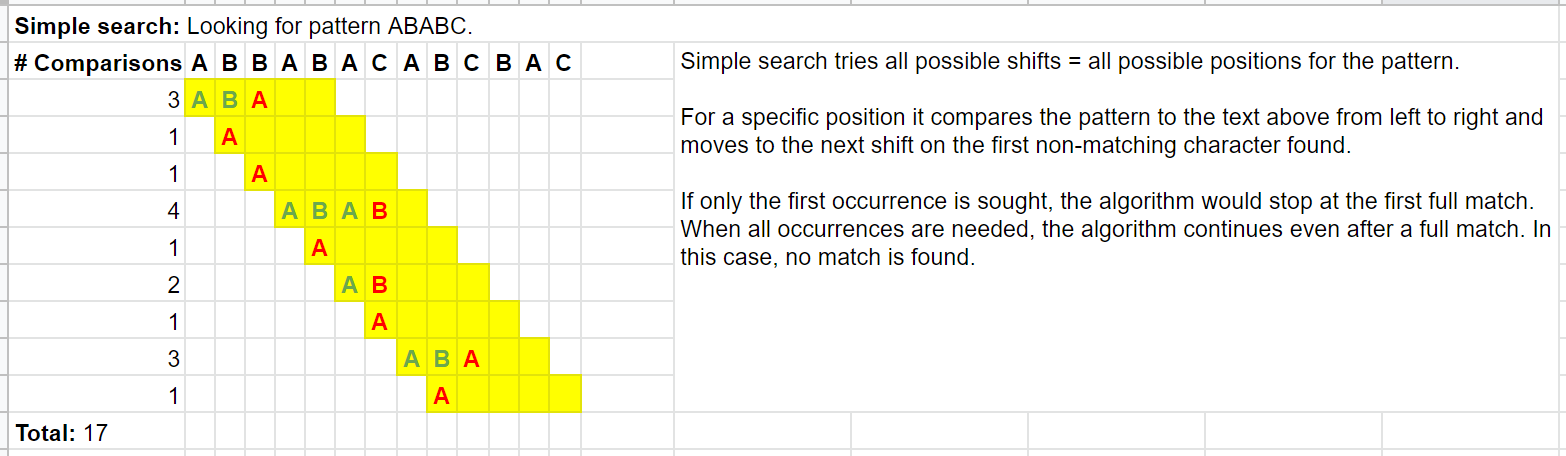
\includegraphics[width=\linewidth]{01/simple_search.png}

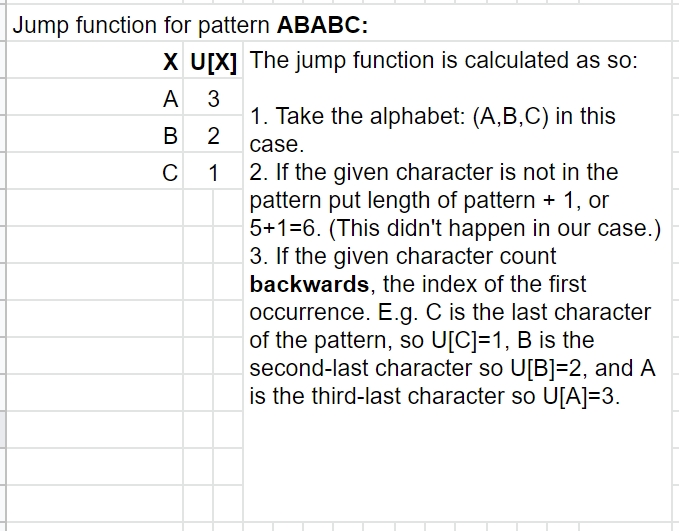
\includegraphics[width=0.5\linewidth]{01/jump_function.png}

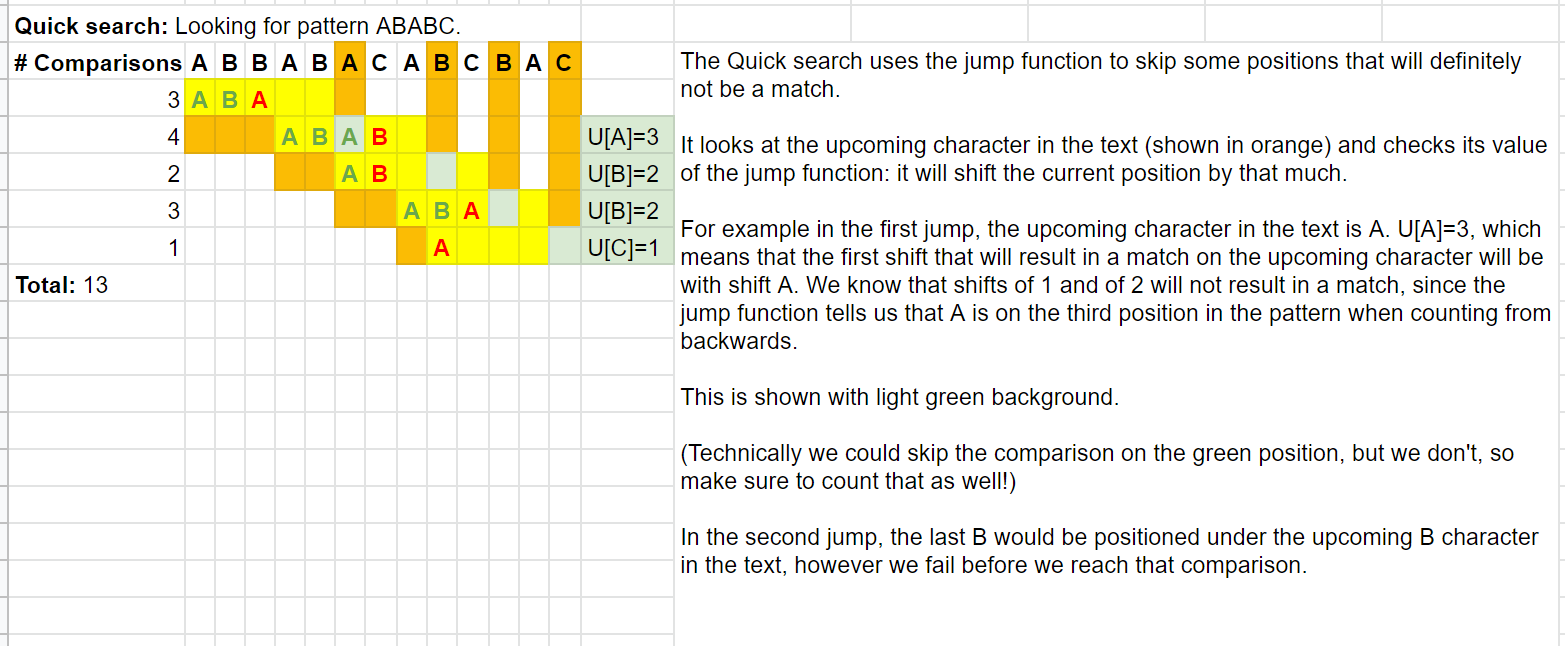
\includegraphics[width=\linewidth]{01/quick_search.png}\pagebreak
\subsection{Session 1, Exercise 9}

\lineparagraph{Exercise}

Let both the pattern and the text consist of only $0$'s, let the length of the pattern be $m$, while that of the text be $n$. How many comparisons are done...

\begin{enumerate}[a.)]
    \item by Simple search if only the first occurrence of the pattern is sought?
    \item by Simple search if all occurrences of the pattern are needed?
    \item by Quick search if only the first occurrence of the pattern is sought?
    \item by Quick search if all occurrences of the pattern are needed?
\end{enumerate}

\lineparagraph{Solution}

\begin{enumerate}[a.)]
    \item $m$, since the first position is immediately a match.
    \item All positions match. There are $n-m+1$ positions, the pattern will be checked on all characters, so $m(n-m+1)$.
    \item $m$, since the first position is immediately a match.
    \item All positions match. There are $n-m+1$ positions, the pattern will be checked on all characters, so $m(n-m+1)$.
\end{enumerate}

Note:
\begin{itemize}
    \item In this case there is no difference between what Simple search and what Quick search does. Quick search is able to skip \textbf{some} definitely non-matching positions based on a heuristic. In this case, all positions match, there is nothing to skip.
\end{itemize}
\pagebreak
\subsection{Session 1, Exercise 10}

\lineparagraph{Exercise}

Give text $S$ of length $n$ such that for a pattern consisting of $m>2$ $0$'s Simple search uses $O(n)$ comparisons on $S$, independently of $m$.

\lineparagraph{Solution}

If the first character doesn't match every position will fail after $1$ comparison. There will be $n-m+1$ positions, which is $O(n)$, because $n-m+1 \leq{} n+1 \leq{} n+n \leq{} 2n$, constants $c=2$, $n_0=1$ work.

So let's make a text in which no character is a $0$, e.g. all characters are $1$'s, so the first $0$ of the pattern will never match.\pagebreak
\subsection{Sesssion 1, Exercise 11}

Note: this is a hard exercise, using probability theory as well, it is not included in the exam!

\lineparagraph{Exercise}

Prove that the expected running time of Simple search is $O(n)$, when both the text and pattern are random $0$ - $1$ sequences (the bits are independent of each other and probabilities of $0$ and $1$ are both $\frac{1}{2}$). What happens if only the pattern is random?

\lineparagraph{Solution}

The pattern is denoted by $M$ and its length is $m=|M|$, the text is denoted by $S$ and its length is $n=|S|$.

Let's denote with the random variable $t_i$ the number of comparisons made by the Simple search algorithm for a pattern position with a shift of $i$ number of characters.

Then, in total the number of comparisons made is $\sum\limits_{i=0}^{n-m}t_i$, so the expected number of comparisons is $E(\sum\limits_{i=0}^{n-m}t_i)$.

$E(\sum\limits_{i=0}^{n-m}t_i) = \sum\limits_{i=0}^{n-m}E(t_i)$, due to the Linearity of Expectation. It is important to remember, that this holds true even when the variables are correlated, like in our case!

Now, the only thing left to find is $E(t_i)$.

For a given position $k$ in the pattern, the probability of it matching the current position in the text, or $P(S[k+i] = M[k])$ is $\frac{1}{2}$, since both the pattern and the text is random, and they match for $S[k+i] = M[k] = 0$ and $S[k+i] = M[k] = 1$ while not match for $S[k+i] = 0, M[k] = 1$ and $S[k+i] = 1, M[k] = 0$, all four of these happen with $\frac{1}{4}$ probability, and two of these are the desired.

Now, the comparisons are made up until the point one of them fails, and we care about the number of them. This would be a geometric distribution, if the number of possible positions would be infinite. While this is not true, since the pattern and the text are both finite, since we only care about an upper bound, we can over-estimate the expectation value with the geometric distribution's expectation value.

$E(t_i) \leq{} \sum\limits_{j=1}^{\infty}j2^{-j} = 2$.

Then we plug this back in:

$E(\sum\limits_{i=0}^{n-m}t_i) = \sum\limits_{i=0}^{n-m}E(t_i) \leq{} \sum\limits_{i=0}^{n-m}2 = 2(n-m+1) \in{} O(n)$.

When only the pattern is random, the only thing changing here is how we calculate $P(S[k+i] = M[k])$. If the text's character is a $0$, or $S[k+i]=0$ then the probability of a random $M[k]$ matching it is $\frac{1}{2}$, when $M[k]=0$. Similarly, if the text's character is a $1$, or $S[k+i]=1$ then the probability of a random $M[k]$ matching it is $\frac{1}{2}$, when $M[k]=1$. So the probability is the same and the same result holds here as well.\pagebreak
\subsection{Session 1, Exercise 12}

Note: this is a hard exercise, it is not included in the exam!

\lineparagraph{Exercise}

Algorithm A solves the problem of pattern matching for $0$ - $1$ sequences, in case of pattern of $m$ bits and text of $n$ bits it uses $T(n, m)$ steps to give all occurrences of the pattern (in increasing order). How can this be used to find all occurrences of a length $m$ pattern in a length $n$ text over an arbitrary alphabet $\Sigma$ using $O((n + T(n, m))log_2|\Sigma|)$ time?

\lineparagraph{Solution}

Let's just say that $O((n + T(n, m))log_2|\Sigma|)$ is suspiciously specific. Especially the $log_2|\Sigma|$ part indicates that we should encode the alphabet in binary form, then a length of an original character in binary will be $log_2|\Sigma|$ in this new alphabet.

However, an issue with this approach will be, that only whole-character shifts should be allowed. We can not allow the algorithm to shift the pattern by half a binary-encoded character's length and find a match there. There is another issue, where this would also result in $T(log_2|\Sigma|n, log_2|\Sigma|m)$ runtime for $A$ and we have no idea about the inner workings of $T$ to somehow estimate this using $T(n,m)$.

Both of these issues will be solved, if we instead create $k = \lceil log_2|\Sigma| \rceil$ number of different pattern matching tasks, and the $i$th task will contain the original task's characters replaced by their $i$th bits.

Now if we let the algorithm find all the occurrences, if it finds let's say an occurrence with shift $a$ in all of the $k$ tasks, that means that all of the bits of the characters match, so the original pattern matches the original text with shift $a$ as well!

To keep track of the results of the $k$ tasks, we create an array $Z$ of length $n$, initialized with $0$'s at the beginning. If the algorithm on the $i$th task finds an occurrence with shift $a$, it increments $Z[a]$ with $1$. Then, at the end when all algorithms finished we read $Z$ and if the value at position $a$ is $k$ that means that all of the $k$ tasks found that as a match, so the original pattern matches with shift $a$ as well.

Finally, the number of steps required to run $A$ on $k$ tasks with the same length as the original string but in binary is $kT(n, m)$, while initializing and incrementing the $Z$ array (of size $n$) is at most $nk$, so in total we are at $O((n+T(n,m))k)$ steps, which is $O((n+T(n,m))log_2|\Sigma|)$.
\pagebreak

\section{Finite Automata}
\subsection{Session 2, Exercise 01}

\lineparagraph{Exercise}

Let $\Sigma=\{0,1\}$. Give a deterministic finite automaton that accepts the words that contain an even number of zeros and an odd number of ones.

\lineparagraph{Solution}

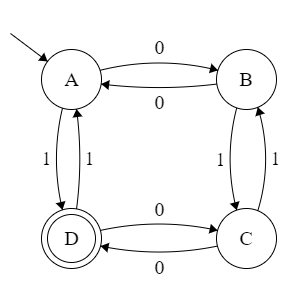
\includegraphics[width=0.4\linewidth]{02/2_1.png}

Proof:

Let's look at what the states mean:

\begin{itemize}
    \item A: State $A$ represents words that contain an even number of $0$'s and $1$'s.
    \item B: State $B$ represents words that contain an odd number of $0$'s and an even number of $1$'s.
    \item C: State $C$ represents words that contain an odd number of $0$'s and an odd number of $1$'s.
    \item D: State $D$ represents words that contain an even number of $0$'s and an odd number of $1$'s.
\end{itemize}

Let's look at the starting state and the accepting and rejecting states:

\begin{itemize}
    \item The starting state is the state that should represent the empty string. The empty string contains zero $0$'s and zero $1$'s, and zero is even, which is represented by $A$, so the starting state is $A$.
    \item The only accepting state is $D$, since we want to accept words that contain an even number of zeros and an odd number of ones, which are represented by $D$.
    \item $A$,$B$ and $C$ are rejecting states, since they represent words that are not in the desired language.
\end{itemize}

Let's look at the transitions:

\begin{itemize}
    \item Transitions triggered by a $0$ input are $A\rightarrow{}B$, $B\rightarrow{}A$, $C\rightarrow{}D$, $D\rightarrow{}C$. In these cases the parity of the $1$'s doesn't change, while the parity of the $0$'s is inverted. If we look back on what the states represent we can verify in all $4$ cases that this is the case.
    \item Transitions triggered by a $1$ input are $A\rightarrow{}D$, $D\rightarrow{}A$, $B\rightarrow{}C$, $C\rightarrow{}D$. In these cases the parity of the $0$'s doesn't change, while the parity of the $1$'s is inverted. If we look back on what the states represent we can verify in all $4$ cases that this is the case.
\end{itemize}\pagebreak
\subsection{Session 2, Exercise 2}

\lineparagraph{Exercise}

Let $\Sigma=\{0,1\}$. Give a deterministic finite automaton that accepts the words that contain an even number of zeroes, while the number of ones is divisible by three.

\lineparagraph{Solution}


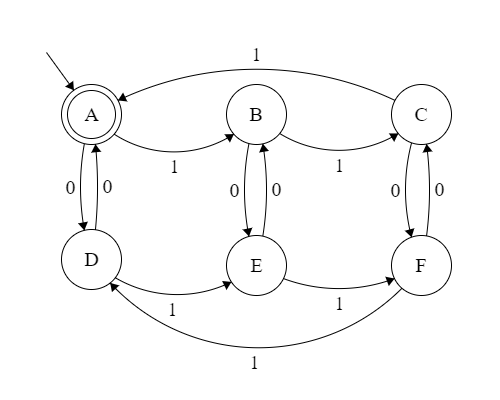
\includegraphics[width=0.5\linewidth]{02/2_2.png}

Proof:

Let's look at what the states mean:

\begin{itemize}
    \item A: State $A$ represents words that contain an even number of $0$'s and the number of $1$'s is in the form $3k$ (divisible by three).
    \item B: State $B$ represents words that contain an even number of $0$'s and the number of $1$'s is in the form $3k+1$.
    \item C: State $C$ represents words that contain an even number of $0$'s and the number of $1$'s is in the form $3k+2$.
    \item D: State $D$ represents words that contain an odd number of $0$'s and the number of $1$'s is in the form $3k$ (divisible by three).
    \item E: State $E$ represents words that contain an odd number of $0$'s and the number of $1$'s is in the form $3k+1$.
    \item F: State $F$ represents words that contain an odd number of $0$'s and the number of $1$'s is in the form $3k+2$.
\end{itemize}

Let's look at the starting state and the accepting and rejecting states:

\begin{itemize}
    \item The starting state is the state that should represent the empty string. The empty string contains zero $0$'s and zero $1$'s, and zero is even and also divisible by three, which is represented by $A$, so the starting state is $A$.
    \item The only accepting state is $A$, since we want to accept words that contain an even number of zeros and the number of ones is divisible by three in them, which are represented by $A$.
    \item The other states are rejecting states, since they represent words that are not in the desired language.
\end{itemize}

Let's look at the transitions:

\begin{itemize}
    \item Transitions triggered by a $0$ input are $A\rightarrow{}D$, $D\rightarrow{}A$, $B\rightarrow{}E$, $E\rightarrow{}B$, $C\rightarrow{}F$, $F\rightarrow{}C$. In these cases the parity of the $1$'s doesn't change, while the parity of the $0$'s is inverted. If we look back on what the states represent we can verify in all $6$ cases that this is the case.
    \item Transitions triggered by a $1$ input:
    \begin{itemize}
        \item $A\rightarrow{}B$ and $D\rightarrow{}E$ move from states that have seen $3k$ $1$'s to states that have sen $3k+1$ $1$'s (the remainder goes from $0$ to $1$).
        \item $B\rightarrow{}C$ and $E\rightarrow{}F$ move from states that have seen $3k+1$ $1$'s to states that have sen $3k+2$ $1$'s (the remainder goes from $1$ to $2$).
        \item $C\rightarrow{}A$ and $F\rightarrow{}D$ move from states that have seen $3k+2$ $1$'s to states that have sen $3k$ $1$'s (the remainder goes from $2$ to $0$).
    \end{itemize}
\end{itemize}\pagebreak
\subsection{Session 2, Exercise 03}

\lineparagraph{Exercise}

Let $\Sigma=\{0,1\}$. Give a deterministic finite automaton that accepts the words that contain at least three $1$'s.

\lineparagraph{Solution}
\pagebreak
\subsection{Session 2, Exercise 04}

\lineparagraph{Exercise}

Let $\Sigma=\{0,1\}$. Give a deterministic finite automaton that accepts the words that do not contain the subword $001$.

\lineparagraph{Solution}

When dealing with \textbf{deterministic} finite automatons, a useful trick to keep in mind: sometimes it is easier to give a DFA for the complementer of the language, and then a DFA for the original language can be quickly created.

IMPORTANT: This trick only works for \textbf{deterministic finite automatons}!!!

\textbf{Step 1}: Create DFA for the complementer of the language:

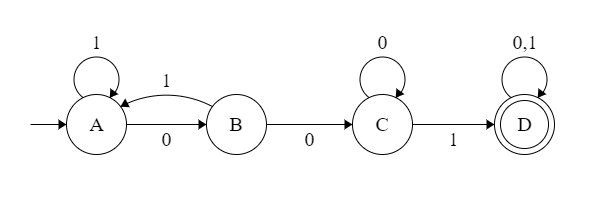
\includegraphics[width=0.6\linewidth]{02/2_4.png}

\textbf{Step 2}: Invert the accept/reject status of the states:

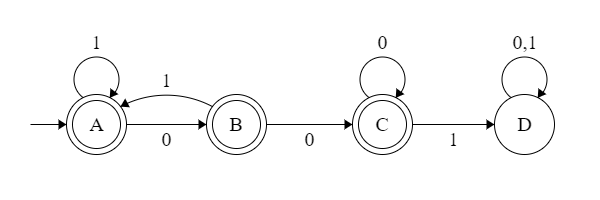
\includegraphics[width=0.6\linewidth]{02/2_4_inv.png}

Proof:

Let's look at what the states mean:

\begin{itemize}
    \item A: State $A$ represents words that end in something that is not a prefix of $001$: they either are the empty string or they end in a $1$; and do not contain $001$ itself.
    \item B: State $B$ represents words that end in $0$.
    \item C: State $C$ represents words that end in $00$.
    \item D: State $D$ represents words that contain $001$.
\end{itemize}

Let's look at the starting state and the accepting and rejecting states:

\begin{itemize}
    \item The starting state is the state that should represent the empty string. The empty string contains no prefix of $001$, so it is represented by $A$.
    \item In the original DFA words that contain $001$ were accepted, which is represented by state $D$, while states $A$,$B$ and $C$ were rejecting.
    \item To get a DFA for the complementer of the language, we simply need to accepts words that we have rejected before and reject words that we have accepted before. This is done by making states $A$,$B$ and $C$ accept, while making state $D$ reject.
\end{itemize}

Let's look at the transitions:

\begin{itemize}
    \item In state $A$, when we read in a $0$ we can move to state $B$, since now the current ending is $0$. However when we read $1$'s, we are not getting closer to finding a $001$ substring (we need the $0$'s first), so we just discard them.
    \item In state $B$, we have the ending $0$. When we read another $0$ in, this results in having the ending $00$, so we can move forward to state $C$, one step closer to finding the substring $001$. However if we read in a $1$, this ruins our progress, since the current ending is now $01$, but we needed a $00$. We can't even stay in state $B$, since we would need a $0$ ending for that, but the last character has been a $1$. We have to move all the way back to state $A$.
    \item In state $C$ the current ending is $00$. If we read in a $1$, that means we just found a $001$ substring, we can move to state $D$! And if we read a $0$ in, while we can't move to state $D$, we can stay in $C$, since the current ending is $000$, or discarding the oldest $0$: $00$, which means we can stay in state $C$.
    \item In state $D$ we have already found the substring, we just read in the remainder of the input, discard it and accept when done.
\end{itemize}\pagebreak
\subsection{Session 2, Exercise 05}

\lineparagraph{Exercise}

Which words are accepted by this automaton? ($\Sigma=\{0,1\}$).

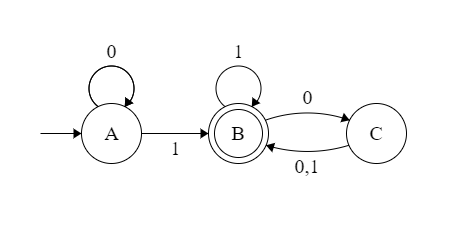
\includegraphics[width=0.5\linewidth]{02/2_5_automaton.png}

\lineparagraph{Solution}
\pagebreak
\subsection{Session 2, Exercise 6}

\lineparagraph{Exercise}

Perform the following for both nondeterministic finite automata.
\begin{enumerate}[a.)]
    \item Give the computation tree of word $baabab$.
    \item Create an equivalent DFA by the procedure studied in class.
    \item Which languages are recognized by these automata?
\end{enumerate}

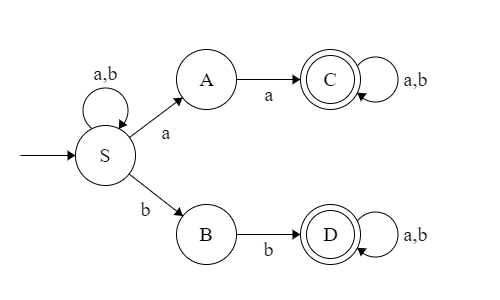
\includegraphics[width=0.5\linewidth]{02/2_6_1_automaton.png}

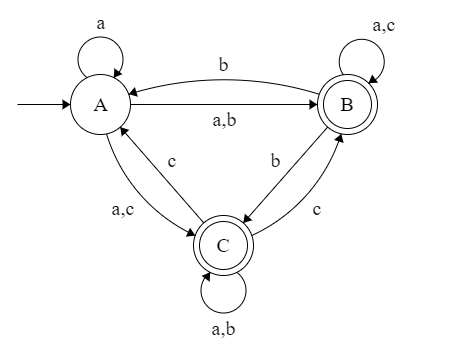
\includegraphics[width=0.5\linewidth]{02/2_6_2_automaton.png}

\lineparagraph{Solution}

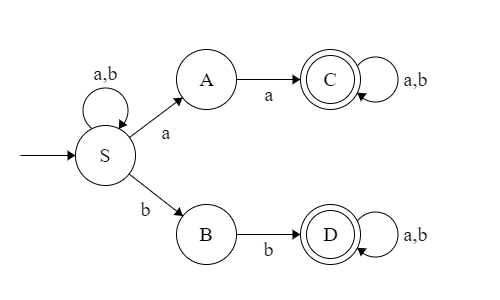
\includegraphics[width=0.5\linewidth]{02/2_6_1_automaton.png}

Give the computation tree of word $baabab$:

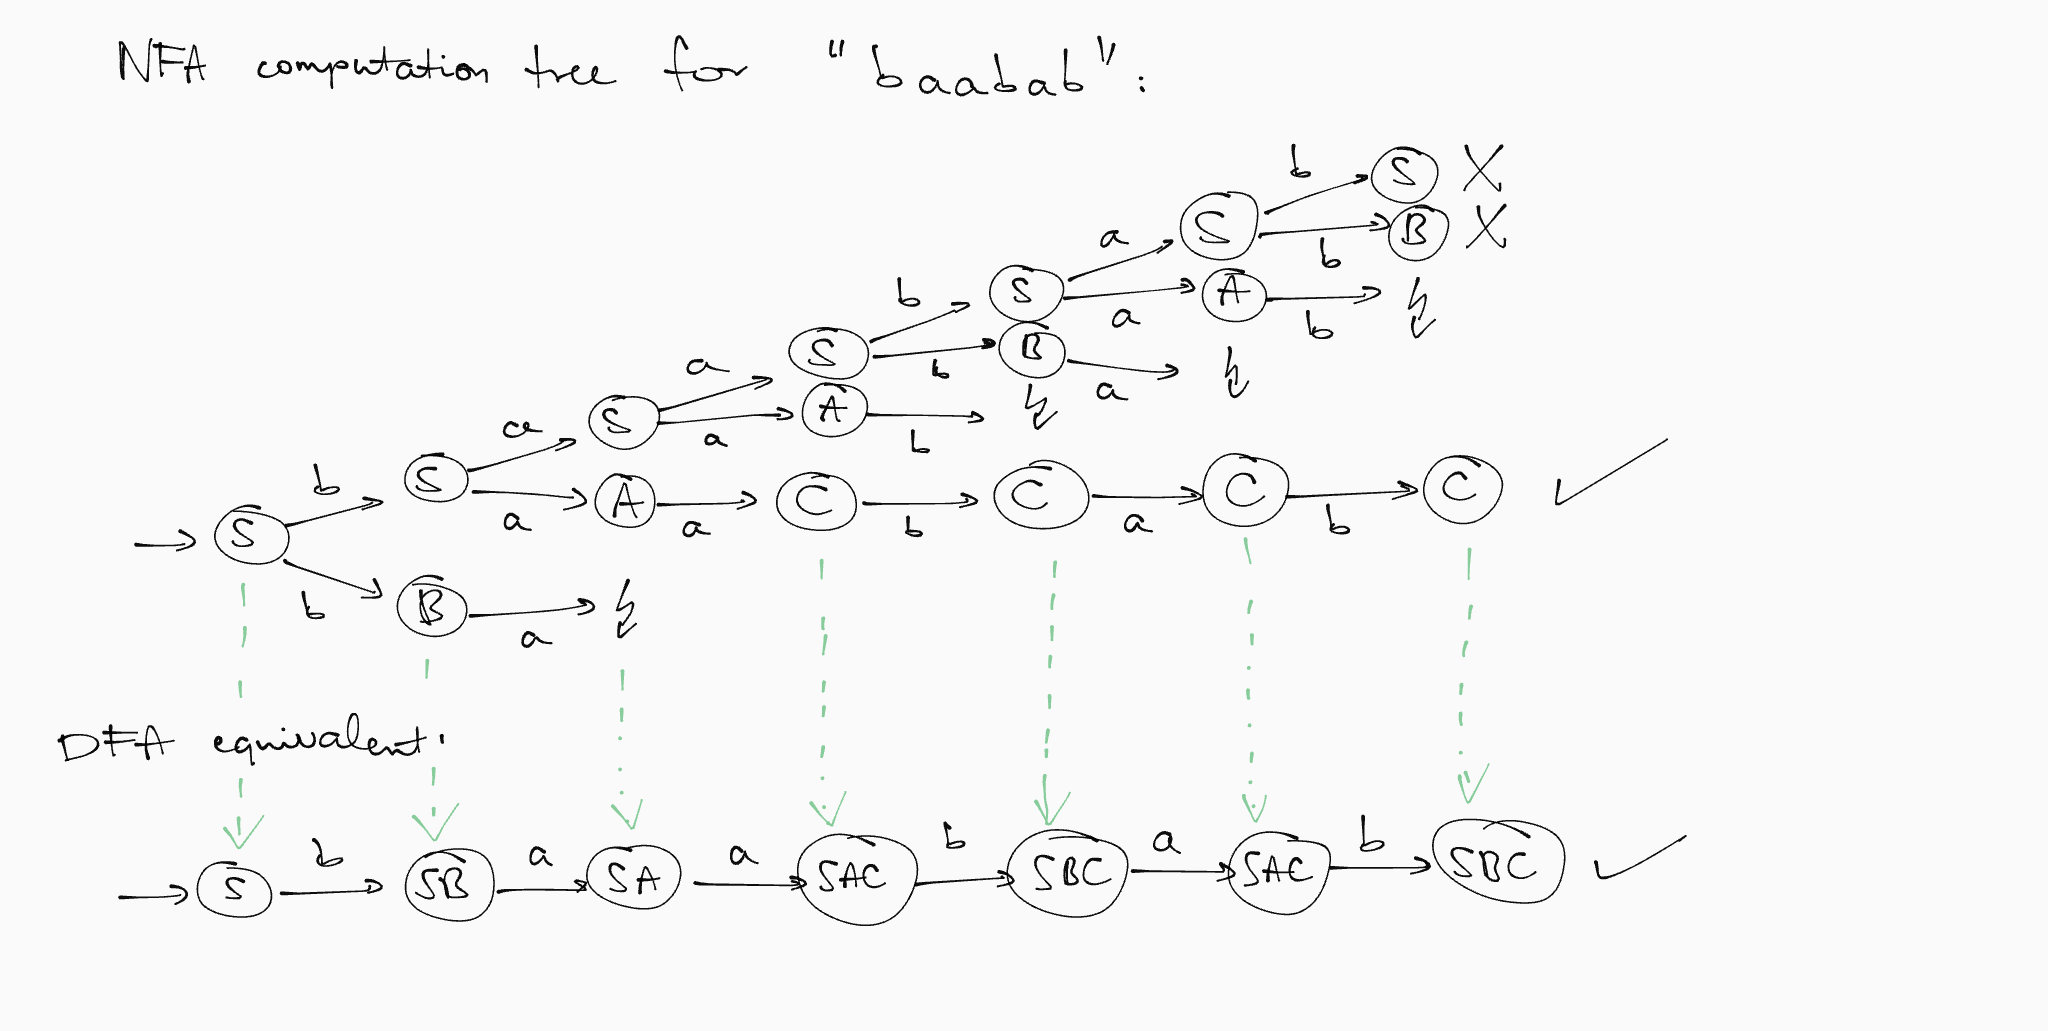
\includegraphics[width=\linewidth]{02/comp_tree_1_nfa_dfa.png}

The word $baabab$ is accepted, since there exists a branch that resulted in an accept state ($C$).

The DFA equivalent computation is also shown in the drawing. We basically follow all branches in ''parallel'', using meta states. We will construct the DFA, that will do a computation like this one:

\textbf{Step 1}

We start with the same starting state as in the NFA: $S$.

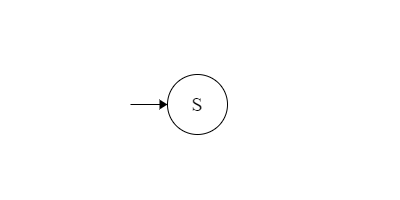
\includegraphics[width=0.5\linewidth]{02/dfa_step_01.png}

\textbf{Step 2}

Then, we check where can we move for an $a$ input from $S$ in the NFA: $S\xrightarrow{a}\{S,A\}$, so we add the $SA$ state for an $a$ transition, and similarly for $S\xrightarrow{b}\{S,B\}$, so we add the $SB$ state for a $b$ transition.

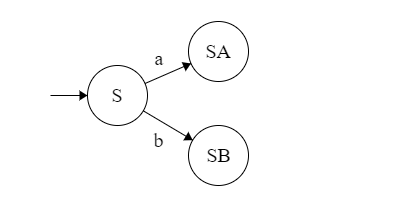
\includegraphics[width=0.5\linewidth]{02/dfa_step_02.png}

Check back on the DFA equivalent on the drawing above! You will notice the state $SB$ as the second step.

\textbf{Step 3}

And we continue the same thing for the new states:

Where does $SA$ move for an input character of $a$? The transitions from $S$ and from $A$ for input $a$ are: $S\xrightarrow{a}\{S,A\}$ and $A\xrightarrow{a}\{C\}$, so together they move to state $SAC$.

Where does $SA$ move for an input character of $b$? The transitions from $S$ and from $A$ for input $b$ are: $S\xrightarrow{b}\{S,B\}$ and $A\xrightarrow{b}\{\}$, so together they move to state $SB$.

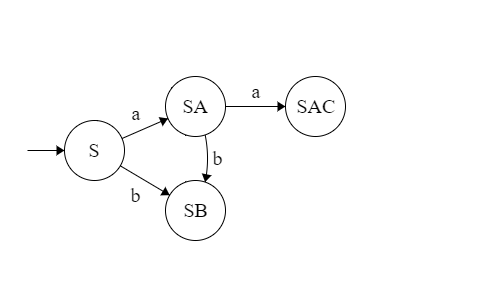
\includegraphics[width=0.7\linewidth]{02/dfa_step_03.png}

The process is the same: find a state that does not have all transitions defined (for $a$ and for $b$ input as well), check where their basis states transition in the NFA for the given input and add it as a transition. If the resulting state does not exist, add the state.

When no new states are added and all states transitions are fully defined the process is done.

\textbf{Step 4}

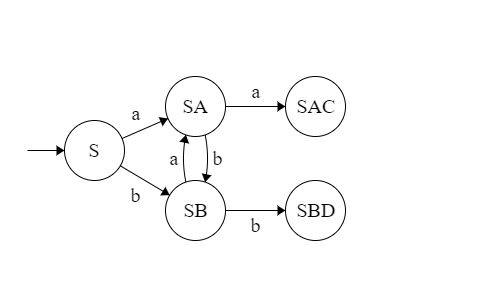
\includegraphics[width=0.7\linewidth]{02/dfa_step_04.png}

\textbf{Step 5}

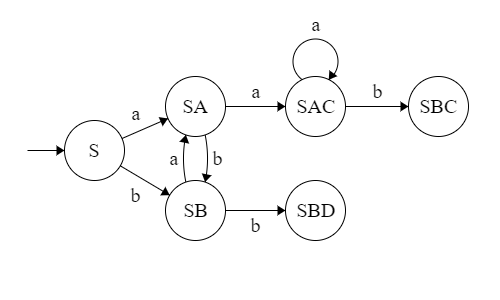
\includegraphics[width=0.7\linewidth]{02/dfa_step_05.png}

\textbf{Step 6}

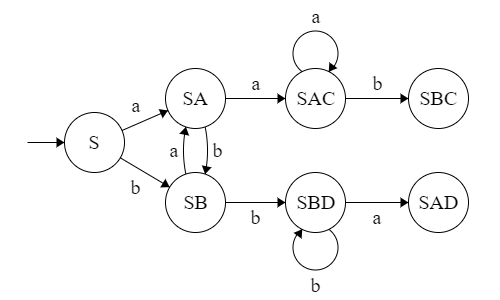
\includegraphics[width=0.7\linewidth]{02/dfa_step_06.png}

\textbf{Step 7}

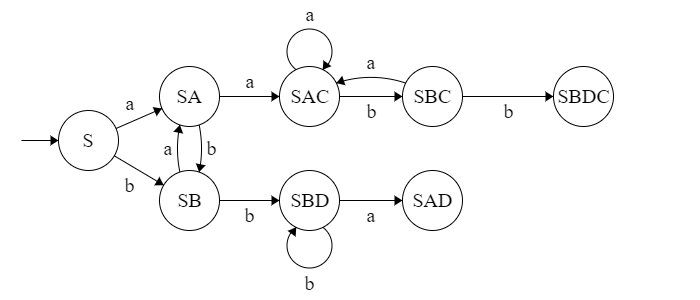
\includegraphics[width=0.9\linewidth]{02/dfa_step_07.png}

\textbf{Step 8}

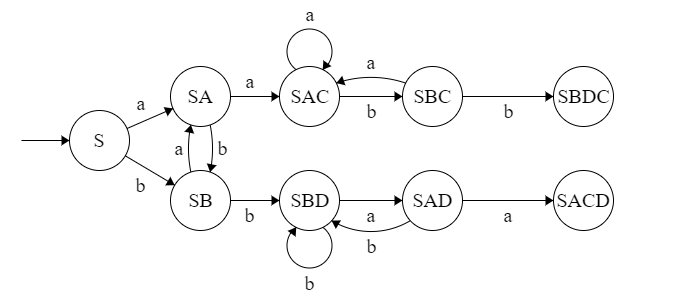
\includegraphics[width=0.9\linewidth]{02/dfa_step_08.png}

\textbf{Step 9}

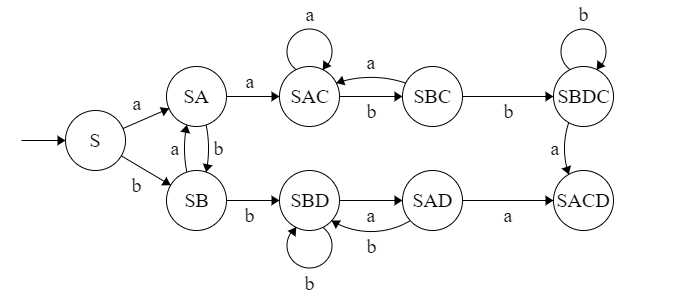
\includegraphics[width=0.9\linewidth]{02/dfa_step_09.png}

\textbf{Step 10}

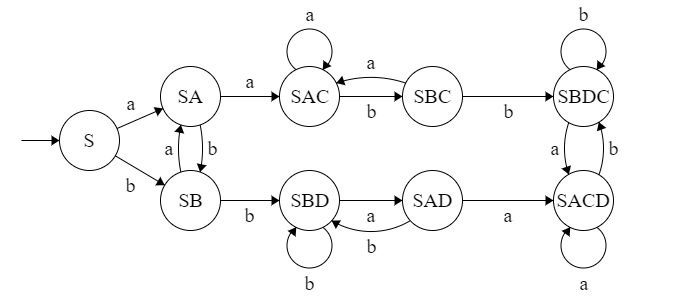
\includegraphics[width=0.9\linewidth]{02/dfa_step_10.png}

\textbf{Step 11}

Finally, define the accepts states: Any state that contains an original accept state (in this case $C$ or $D$) will be an accepting state:

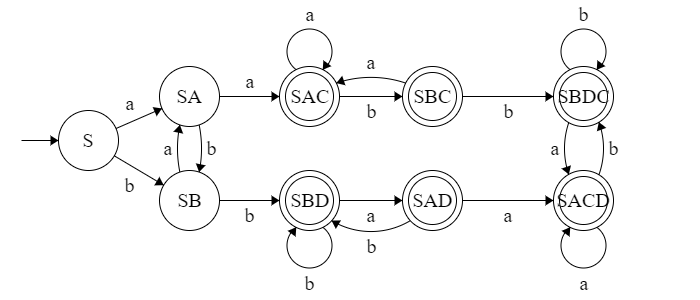
\includegraphics[width=0.9\linewidth]{02/dfa_step_11.png}

\textbf{Note}

By the way, the automaton can be simplified, like this:

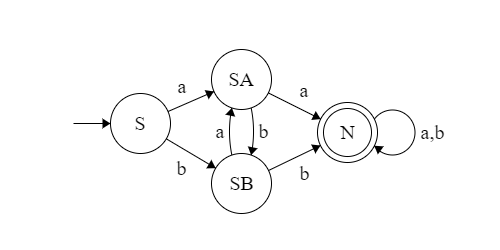
\includegraphics[width=0.7\linewidth]{02/dfa_final.png}

Since the moment we reach any of the accepts states, we will never leave them.


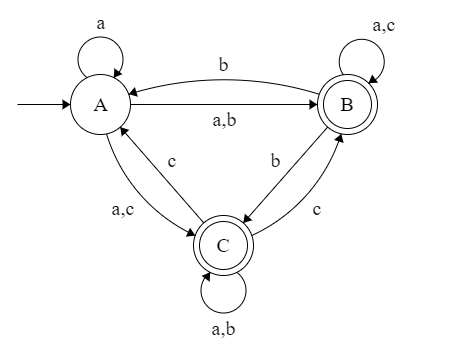
\includegraphics[width=0.5\linewidth]{02/2_6_2_automaton.png}

TODO\pagebreak
\subsection{Session 2, Exercise 7}

\lineparagraph{Exercise}

Give a nondeterministic finite automaton that accepts those words that have 10100 as subword.

\lineparagraph{Solution}

The key to solving this exercise using a nondetermnistic automaton is to create a delayed start on the starting state by introducing a 0,1 loop on it:

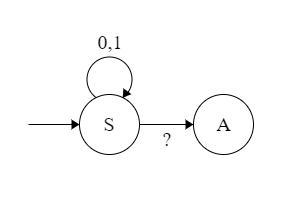
\includegraphics[width=200px]{02/wait_to_start.png}

This will "eat up" some prefix of the input word before allowing the computation to proceed to state A. Whatever we put in place of the ? on the leaving transition will be a nondeterministic choice for the automaton.

The next step is to add the success path to the automaton which contains the string we want to have as a subword: 10100.

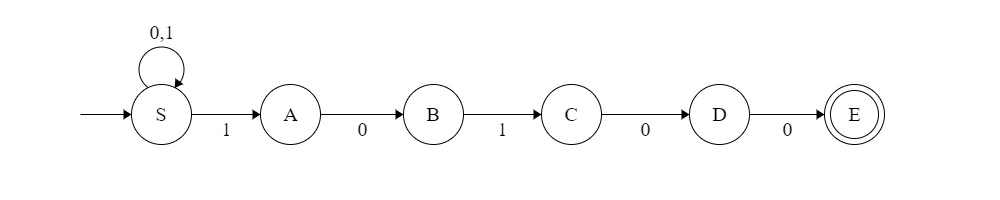
\includegraphics[width=\linewidth]{02/success_path.png}

Then finally, let's allow "eating up" any remaining suffix of the word as well:

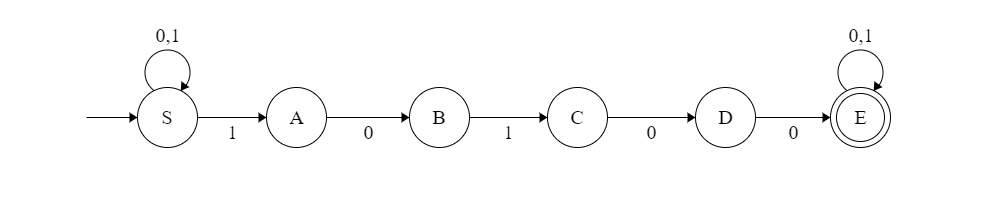
\includegraphics[width=\linewidth]{02/10100.png}

Some observations:

\begin{itemize}
    \item Firstly, this is a nondeterministic finite automaton: Notice how in state $S$, for an input character of $1$ we can either remain in $S$, or move to state $A$.
    \item There are also transitions missing: it is an incomplete finite automaton as well. For example, in state $A$, for an input character of 1, the machine halts (and halting due to a missing transition means rejection, \textbf{regardless of the current state's accept/reject status}.
    \item Notice how visually similar this automaton is to the regular expression for the same language: $(0+1)^*10100(0+1)^*$.
\end{itemize}

Let's look at an example computation on the word 1110100, which is in the language of the automaton.

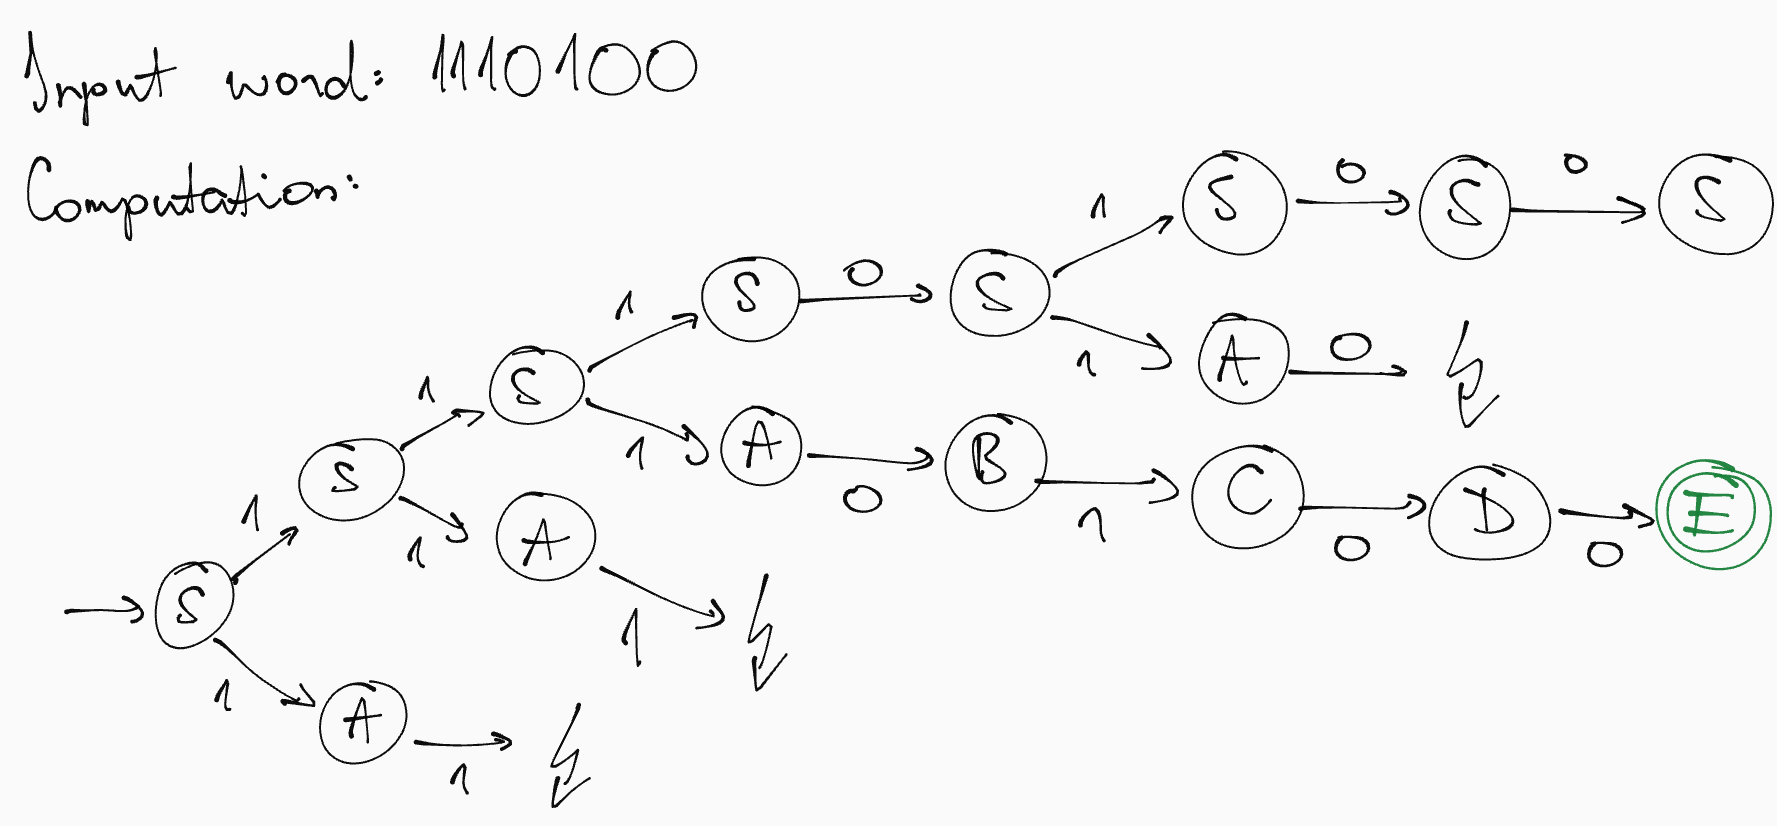
\includegraphics[width=\linewidth]{02/computation_1110100.png}

\begin{itemize}
    \item See, how it tried to leave state $S$ and move to state $A$ many times in different places of the input string? Many times it failed, when the timing was incorrect. Maybe it was too early, when the first two 1's, which are not part of the matching subword were given to it, or it was too late, when the pattern was already gone.
    \item There was already a lazy case, the top branch, which just remained in state $S$ forever, which also could not succeed.
    \item However there only needs to be a single successful branch and it only needs to time its move to state $A$ correctly once: on the third branch it successfully finished in state $E$, which means that the word is accepted, correctly!
    \item Notice how it is only possible to reach state $E$, when the input word contains 10100. We need a 1 to move from $S$ to $A$, then we need a consecutive $0$ to move from $A$ to $B$, then we need a consecutive $1$ to move from $B$ to $C$, then we need a consecutive $0$ to move from $C$ to $D$, then we need another consecutive $0$, to move from $D$ to $E$.
    \item When the timing is just right and we catch the beginning of the pattern we can ''sail smoothly'' towards $E$.
\end{itemize}

When you are on the exam, you will need to give some sort of proof that the automaton you wrote up does what the exercise is asking you to do. For this exercise this is how a proof like this might look like:

\textbf{Proof:}

1. Let's look at the states of the automaton:
What the different states mean and why their transitions are correct.
\begin{itemize}
    \item State $S$ is the starting state. Here, we non-deterministically wait to start our computation, using the $0$,$1$ loop. Since the first character of the pattern we seek is a $1$, on an input character of $1$, the automaton can decide to move to state $A$.
    \item State $A$ represents the information "already read the first character of the pattern". Here, we allow a transition to state $B$ if the second character of the pattern comes, which is a $0$. However, the transition for an input of $1$ is missing, which means that the computation (on that branch) will halt. This is correct, because the pattern's characters must be consecutive.
    \item States $B$, $C$ and $D$ work similaly: they represent the next character recognized from the pattern we seek and we only allow a transition for the upcoming character from the pattern to move forward, towards $E$.
    \item Finally, state $E$ represents "pattern found". This means that we can accept the word, furthermore, any further input characters are allowed, since the pattern can be anywhere in the word.
\end{itemize}

2. Let's look at the accepted and rejected words of the automaton:

Any word that contains the pattern 10100 will be accepted, because the automaton on the (single) accepting branch of the computation first non-deterministically reads the prefix of the word before the pattern, then transitions from $S$, to $E$ using the consecutive characters of the pattern, then finally in state $E$ further characters can be read (the remaining suffix of the word) and the word will be accepted.

Any word that does not contain the pattern 10100 can not reach state $E$, because each step towards $E$ requires the next character of the pattern to be present consecutively in the word. There is correct timing to leave $S$, no computational branch can end up in $E$, so the word will be rejected.

\textbf{(End of proof.)}

(Due to time limits on the exam, it is okay to not use full sentences like I did above, abbreviate things, etc.)

It is important when doing these proofs, that you do not use a specific input word as an example, but generalize to any possible words, like the proof above.

\lineparagraph{Deterministic solution}

This exercise allows us to truly appreciate nondeterministic automata, since it made it really easy for us to come up with a design for a given subword.

However, the task is also possible with a deterministic automaton (it must be, since we can convert any NFA into a DFA, but there is an even easier method to obtain a DFA, than the general conversion algorithm). This is not part of the task, but nice to see how it works as well.

Step 1: Get rid of loop on the starting state, we need to be deterministic now.

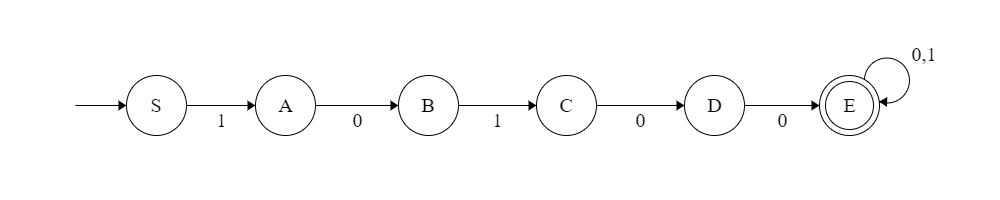
\includegraphics[width=\linewidth]{02/det_10100_1.png}

Step 2: Put in the missing transitions, states $S$-$D$ all miss 1 of them.

The main idea here is that the missing transitions are failures in recognizing the next character of the pattern at the current position. How big of a failure it is depends on what the pattern we have found so far is and how much of it can be salvaged when we add the incorrect character at the end.

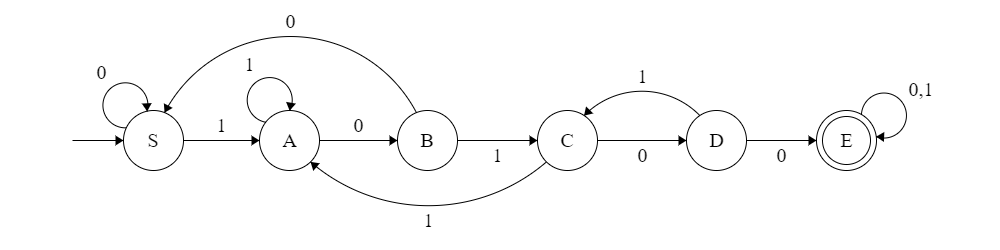
\includegraphics[width=\linewidth]{02/det_10100_2.png}

\begin{itemize}
    \item When we are in state $S$, the pattern we have found so far is nothing. Until we read $0$'s we remain in state $S$, since the first character of the pattern is a $1$.
    \item When we are in state $A$, the pattern we have found so far is ''$1$''. If we read another $1$ now, we now have ''$11$''. The pattern is ''$10100$'', so that second $1$ character can still turn out to be the beginning of the pattern, so we need to remember that we have a ''$1$'' and thus stay in state $A$.
    \item When we are in state $B$, the pattern we have found so far is ''$10$'', if we read a $0$ in now, that makes it a ''$100$''. Unfortunately, there is no salvaging this: not ''$100$'', not ''$00$'' and not even a single ''$0$'' is useful for us, neither of them are the prefixes of the pattern ''$10100$''. We need to scratch everything and go back to state $S$.
    \item When we are in state $C$, the pattern we have found so far is ''$101$''. If we read a $1$ now, that makes it ''$1011$''. The possible suffixes to remember here are ''$011$'', ''$11$'' and ''$1$''. In general we always need to keep the longest one that is still a prefix of the pattern: in this case, that is ''$1$'', which is represented by state $A$, so we move back there.
    \item When we are in state $D$, the pattern we have found so far is ''$1010$''. If we read a $1$ now, that makes it ''$10101$''. This is great news, because we can actually just forget the first two characters and we can still keep the remaining ''$101$'', which is the first three characters of the pattern! Not much is lost, ''$101$'' is represented by state $C$, so we can move there.
\end{itemize}\pagebreak
\subsection{Session 2, Exercise 08}

\lineparagraph{Exercise}

Prove that the language that consists o those words that have two $1$'s such that the number of $0$'s between them is divisible by four, is regular. (There could be several $1$'s between the two chosen $1$'s, besides the $4k$ $0$'s.)

\lineparagraph{Solution}
\pagebreak
\subsection{Session 2, Exercise 09}

\lineparagraph{Exercise}

Design a finite automaton that accepts positive rational numbers written in decimal form. ($\Sigma$ contains the decimal point and digits $0,1,2,3,4,5,6,7,8,9$.) The number to be accepted is either an integer without decimal point (e.g. $123$), or it contains a decimal point. In this latter case numbers without integer part or fractional part must also be accepted, but at most one of these parts may be missing. (For example, $123.456$, $123.$ and $.456$ are all accepted, but a single decimal point is not.) It is also requested that a number cannot begin with dummy $0$'s, however $0.456$ is OK.)

\lineparagraph{Solution}
\pagebreak
\subsection{Session 2, Exercise 10}

\lineparagraph{Exercise}

Let $\Sigma = \{0, 1\}$. The sequences are considered as binary numbers. Give a finite automaton that accepts exactly those words that represent numbers divisible by three in binary form. Take into consideration that a number does not begin with $0$, except for number zero itself, and that the input number is read beginning with the most significant digit.

\lineparagraph{Solution}

Any automaton that we design will work by reading the input binary string from left to right. We will want to keep track of the remainder of the current binary number after each 0 or 1 we read. The question is how do we update this remainder when the next input character comes? First, let's do a simpler task, just keeping track of the number itself and updating it as we go.

\begin{itemize}
    \item For example, let's say that so far we have read the the ''$101$'' binary string on the input. That is a $5$ in decimal form.
    \item Let's say the next character is also a $1$, so now the current string is ''$1011$'', or in decimal form $11$.
    \item This was achieved by shifting the string ''$101$'' to the left and adding a ''$1$'' as the least significant character.
    \item A left shift in binary corresponds to multiplication by $2$ in decimal, and then if the next character is a $1$, we just need to add $1$ to the decimal value as well. So in our example, $5*2 + 1 = 11$.
    \item In general, if we read a binary number from left to right, to calculate its decimal value, we simply multiply the current decimal value by $2$, and if the bit we read was a $1$, we add a $1$ and continue to the next bit.
\end{itemize}
 
If we don't care about the entire number, just its remainder when divided by $3$, we can do the same calculation, but modulo $3$.

If the current number is divisible by $3$, or in the form $3k$, and the next binary character is a $0$, then to update we do $3k*2+0 = 6k$, which means that the updated number will still be divisible by $3$.

If the next binary character is a $1$, then to update we do $3k*2+1=6k+1=3*(2k)+1$, which means that the updated number has a remainder of $1$ when divided by $3$.

We can represent these statements by the following two transitions from state $3k$:

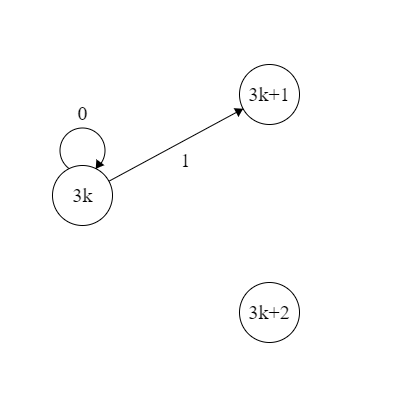
\includegraphics[width=250px]{02/modulo_1.png}

If the current number has a remainder of $1$, when divided by $3$, or in the form of $3k+1$, and the next binary character is a $0$, then to update we do $(3k+1)*2+0=6k+2=3*(2k)+2$, which means that the updated number has a remainder of $2$, when divided by $3$.

If the next binary character is a $1$, then to update we do $(3k+1)*2+1=6k+3=3*(2k+1)$, which means that the updated number is divisible by $3$.

We can represent these statements by the additional two transitions from state $3k+1$:

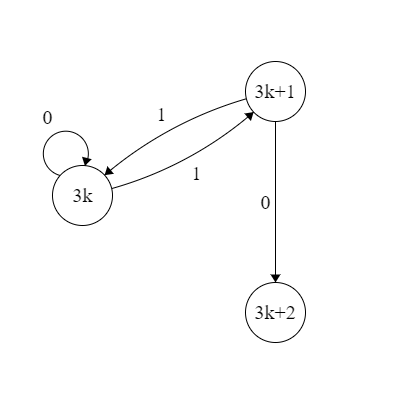
\includegraphics[width=250px]{02/modulo_2.png}

Finally, if the current number has a remainder of $2$, when divided by $3$, or in the for of $3k+2$, and the next binary character is a $0$, then to update we do $(3k+2)*2+0=6k+4=3*(2k+1)+1$, which means that the updated number has a remainder of $1$, when divided by $3$.

If the next binary character is a $1$, then to update we do $(3k+2)*2+1=6k+5=3*(2k+1)+2$, which means that the updated number has a remainder of $2$, when divided by $3$.

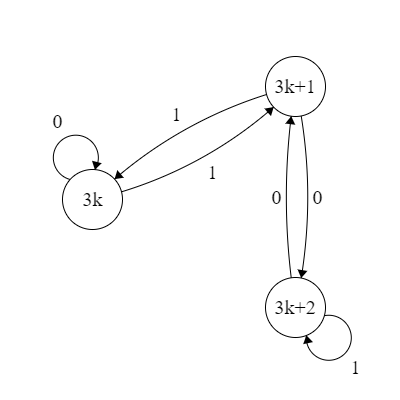
\includegraphics[width=250px]{02/modulo_3.png}

If you want to try this automaton, come up with any decimal number, turn it into binary form and calculate its remainder by $3$, by applying the transitions above using its binary form as input. The starting state should be $3k$, since when we have not read anything in yet, so we want to start from a state that is equivalent to the number $0$, which is divisible by $3$.

I however, did not mark a starting state yet on this image, because there is one additional statement to keep in mind: ''Take into consideration that
a number does not begin with $0$, except for number zero itself.''. This means that we do not consider any string longer than 1 characters starting with a $0$ a number, much less a number that is divisible by $3$, so we need to reject these words.

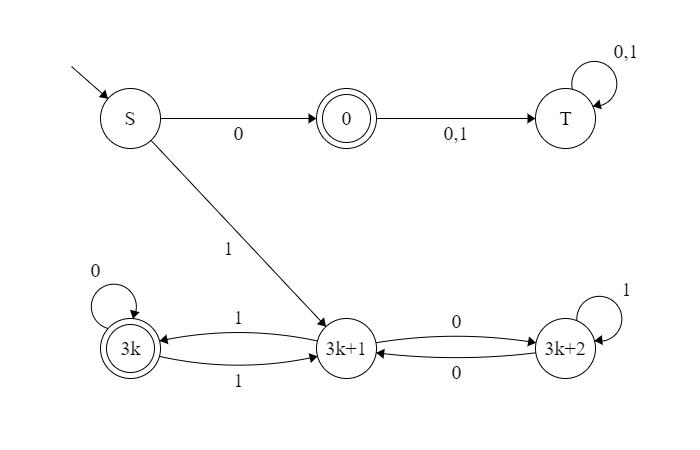
\includegraphics[width=\linewidth]{02/modulo_final.png}

Now, if this was an exam, here is how to prove that this accepts the language: (Basically everything I just said, but in a shortened form.)

\textbf{Proof:}

1. Let's explain what the different states mean and that their transitions are correct:

\begin{itemize}
    \item $S$ is the starting state. If we read a $0$ in, we move to a state dedicated to the number $0$. If we read a $1$ in, we move to the state that represents binary numbers, that give a remainder of $1$ when divided by $3$, which is true for the (binary) number $1$.
    \item The only word for state $0$ is $0$ itself, this is divisible by $3$ and is accepted. If we read anything else after a $0$ that is an incorrectly formatted number and moves to a trap state $T$ which rejects it.
    \item The states $3k$, $3k+1$ and $3k+2$ represent the 3 remainder classes of division by $3$. When a new character is read on the input, we update the remainder class with multiplying by $2$ (binary shift) and adding the $0$ or $1$ bit we just read. We can see that the transitions are correct, since:
    \begin{itemize}
        \item $3k*2+0 = 3*(2k)$
        \item $3k*2+1 = 3*(2k)+1$
        \item $(3k+1)*2+0 = 3*(2k)+2$
        \item $(3k+1)*2+1 = 3*(2k+1)$
        \item $(3k+2)*2+0 = 3*(2k+1)+1$
        \item $(3k+2)*2+1 = 3*(2k+1)+2$
    \end{itemize}
\end{itemize}

2. Let's explain that the correct words are accepted and the words not in the language are rejected:

The words in the language are any numbers that are divisible by $3$, which is either the number $0$ or anything that is in the form $3k$, these states are accepting.

A word could be outside of the language due to being malformed (starting with $0$, but not being $0$ itself), which will be redirected to a trap $T$; or due to not being divisible by $3$, in which case it will land in either $3k+1$ or $3k+2$ and will be rejected there. Finally, the empty string is rejected because it's not a number, which is the only word that will end up in state $S$.

\textbf{(End of proof.)}

Notes:

\begin{itemize}
    \item I ended up making a deterministic automaton here, however the task would allow a non-deterministic one as well. We could get rid of the enitre $T$ state and define no transitions outwards from state $0$. If there is input left to be read in state $0$ the automaton halts due to a missing transition, which rejects the word regardless of the accept/reject status of the current state!
\end{itemize}\pagebreak
\subsection{Session 2, Exercise 11}

\lineparagraph{Exercise}

Let language $L_k$ consist of those word over alphabet $\Sigma=\{a,b\}$ that have character $b$ on the $k^{\text{th}}$ position counting rom backwards. (For example $bbaa\in{}L_3\cap{}L_4$.)

\begin{enumerate}[a.)]
    \item Prove that there exists a nondeterministic automaton of $k+1$ states recognizing language $L_k$ for all $k\geq{}1$.
    \item Prove that every deterministic automaton recognizing $L_k$ has at least $2^k$ states.
\end{enumerate}

\lineparagraph{Solution}
\pagebreak
\subsection{Session 2, Exercise 12}

\lineparagraph{Exercise}

Prove that every NFA can be transformed so that it recognizes the same language, however it has a unique accept state.

\lineparagraph{Solution}
\pagebreak
\subsection{Session 2, Exercise 13}

\lineparagraph{Exercise}

The language $L^R$ is obtained from language $L$ so that every word in $L$ is reversed, that is the characters of the word are written in reverse order. Prove that $L$ is regular $\Leftrightarrow$ $L^R$ is regular.

\lineparagraph{Solution}
\pagebreak

\section{Regular expressions, context-free languages}
\subsection{}
\label{3.1}

\lineparagraph{Exercise}

Let $\Sigma = \{a,b\}$ and let language $L$ consist of words
that contain the same number of $a$'s and $b$'s. Is $L$ regular?

\lineparagraph{Solution}

\textbf{Gut feeling} (This is not yet a proof!)

Not regular.

This language is similar to $a^nb^n$ (studied in the lecture). The
main issue with it will be similar: we would need to remember the difference
of the number of $a$'s and $b$'s we have read in so far and only
accept the word if the difference is $0$ after reading in the entire
word.

For every possible difference, we will need a separate state, however the
difference can be arbitrarily large, while we can only have a finite
number of states using Finite Automata, so it won't be possible
to construct such a machine.

\textbf{Proof}

We will do proof by contradiction:

\begin{itemize}
    \item Let's assume that $L$ is regular.
    \item Then, that means that there exists a Deterministic Finite Automata, that accepts the language $L$.
    \item Let's take one such automata, and name it $M$.
    \item Let's count the number of states in $M$ and name this number $n$.
    \item Now let's list exactly $n+1$ specifically chosen words from the $L$ language: $ab$, $aabb$, $a^3b^3$, $\dots$, $a^{n+1}b^{n+1}$.
    \item Then imagine feeding these $n+1$ words into $M$. For all of them, let $M$ read in the $a$ letters and then stop and take note of which state the word is at the moment, halfway-through the operation.
    \item After reading in $a$, $aa$, $a^3$, $\dots$, $a^{n+1}$, since these are $n+1$ cases, while $M$ only has $n$ states, we can use the \href{https://en.wikipedia.org/wiki/Pigeonhole_principle}{Pigeonhole Principle} and say, that there exists at least two different half-words $a^i$ and $a^j$ $(i\neq{}j)$, for which $M$ arrived at the same state after feeding it these inputs. Let's name this state $S$.
    \item Since $a^ib^i$ is in language $L$, it must be accepted by $M$. This means that when we continue from state $S$ and feed in the $b$'s of the word, the machine must arrive in an accepting state. So there exists a path from state $S$ to an accepting state that is traversed by the input $b^i$.
    \item However, $M$ also arrives in state $S$ when it reads $a^j$. We just noted, that if from $S$ it reads $b^i$ it will arrive in an accept state. If we put these two together, it means that $M$ accepts the word $a^ib^j$, where $i\neq{}j$, which is \textbf{not} in $L$, since it doesn't have the same number of $a$'s and $b$'s.
    \item We stated in the beginning that $M$ is a machine whose language is $L$, however we just found a word that is not in $L$, but accepted by $M$, so this is a contradiction.
\end{itemize}

Notes:

\begin{itemize}
    \item This is symmetric, we could also prove that $M$ accepts $a^ib^j$, for $i\neq{}j$ which is also a contradiction, since that word is also not in $L$.
    \item To put it shortly: the machine cannot distinguish $a^i$ and $a^j$ $(i\neq{}j)$ and since $a^ib^i$ and $a^jb^j$ are accepted, so are $a^ib^j$ and $a^jb^i$, which are not in $L$, which is a contradiction.
    \item Note, that this proof is exactly the same as the proof for language $a^nb^n$ studied in the lecture. This is due to the fact, that these languages are similar, for both of them the issue is keeping track of the number of $a$'s to (eventually or simultaneously) compare them to the number of $b$'s.
    \item It is \textbf{not true}, that ''the proof works because $a^nb^n$ is a subset of $L$''. For example, $a^nb^n$ is also a subset of $\Sigma^*$, which is regular!
\end{itemize}
\pagebreak
\subsection{Session 3, Exercise 2}

\lineparagraph{Exercise}

Let $\Sigma = \{(,)\}$. Prove that the language of properly matched parentheses sequences is not regular.

\lineparagraph{Solution}

Quite similar to \ref{3f1}. The $n+1$ words from $L$, the language of properly matched parentheses to be used are $()$, $(())$, $(^3)^3$, $\dots$, $(^{(n+1)})^{(n+1)}$, so just substitute $a = ($ and $b = )$.\pagebreak
\subsection{Session 3, Exercise 3}

\lineparagraph{Exercise}

Is the language regular, that consists of sequences of $0$'s of a length that is...
\begin{enumerate}[a.)]
\item an even number?
\item an odd number?
\item a perfect square?
\item a power of $2$?
\end{enumerate}

\lineparagraph{Solution}

\subsubsection{Even number of $0$'s}

Regular.

\textbf{Proof 1}: The regular expression $(00)^*$ matches them.

Proof that this regular expression matches the language:

\begin{itemize}
    \item The $^*$ operator allows any number of repeats, even 0.
    \item Inside the $^*$ operator we have two $0$'s, which can be repeated any number of times to match any even number of $0$'s.
    \item The empty string, also known as zero number of $0$'s contains an even number of $0$'s, so it is part of the language. $(00)^*$ matches the empty string, which is correct.
\end{itemize}

\textbf{Proof 2}: The following DFA accepts the language:

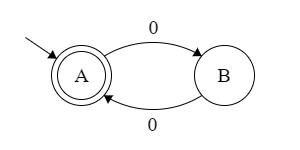
\includegraphics[width=150px]{03/even_zeroes.png}

Proof that this automaton accepts the language:

\begin{itemize}
    \item Words that end up in state $A$ are the words that contain an even number of $0$'s, while words that end up in state $B$ contain an odd number of $0$'s.
    \item The empty string is correctly accepted.
    \item From state $A$, reading another $0$ moves to state $B$, so after reading an even number of $0$'s, if we read one more, now we have an odd number of $0$'s.
    \item And similarly for state $B$.
\end{itemize}

\subsubsection{Odd number of $0$'s}

Regular.

\textbf{Proof 1}: The regular expression $0(00)^*$ matches them.

Proof that this regular expression matches the language:

\begin{itemize}
    \item We have just seen that $(00)^*$ matches an even number of $0$'s.
    \item Adding the $0$ at the front will then match an odd number of $0$'s.
\end{itemize}

\textbf{Proof 2}: The following DFA accepts the language:

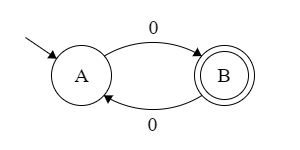
\includegraphics[width=150px]{03/odd_zeroes.png}

Proof that this automaton accepts the language:

\begin{itemize}
    \item This is the same automaton as in the previous exercise, but now the accept state is $B$, to accept an odd number of $0$'s.
\end{itemize}

\subsubsection{A perfect square number of $0$'s}

\textbf{Gut feeling} (This is not yet proof!)

Not regular.

The issue here is going to be, that the length of the accepted words get further and further away from each other as the length of the words increases. We always need to keep track of how far away we are from the next accepted word, how many more $0$'s we need to finally accept. We would need separate states for each of these "$x$ number of $0$'s before we can accept", however $x$ could be arbitrarily large and we only have a finite number of states.

\textbf{Proof}

 Quite similar to \ref{3.1}, the $n+1$ words to use here are of the length of the first $n+1$ square numbers: $0 = 0^{1^2}$, $0000 = 0^{2^2}$, $0^9 = 0^{3^2}$, $0^{16} = 0^{4^2}$, $0^{5^2}$, $0^{6^2}$, $\dots$, $0^{(n+1)^2}$.
 
Then, the finishing of \ref{3.1} is a bit different:

When we find that for an $i\neq{}j$, both $0^{i^2}$ and $0^{j^2}$ end up in the same state $S$, the reasoning is a bit different. Without loss of generality, we can assume that $i<j$. If we were to continue $0^{i^2}$ from state $S$ with $2i+1$ more $0$'s, then the whole input would be $0^{i^2+2i+1} = 0^{(i+1)^2}$, which means that we should accept this word, so from state $S$, for $2i+1$ number of $0$'s we must reach an accept state.

However, this also means that when we continue $0^{j^2}$ (which remember, also arrives in $S$) with $2i+1$ $0$'s, so the word is $0^{j^2+2i+1}$, we will also arrive at the same accept state.

However $j^2+2i+1$ is not a square number. It is between two consecutive square numbers $j^2$ and $(j+1)^2 = j^2+2j+1$, but not equal to either of them:
\begin{itemize}
    \item $j^2 < j^2 + 2i + 1$, since $0<i$.
    \item $j^2 + 2i + 1 < j^2 + 2j + 1$, since $i<j$.
\end{itemize}

Thus, we found a word accepted by $M$, however not in $L$, which is a contradiction.

\subsubsection{A power of $2$}

\textbf{Gut feeling} (This is not yet proof!)

Not regular, the situation is even worse than for square numbers, since powers of $2$ are even further spaced apart as the exponent continues to grow.

\textbf{Proof}

The $n+1$ words to be used are $0^{2^1}$, $0^{2^2}$, $0^{2^3}$, $\dots$, $0^{2^{n+1}}$.

Then similarly to the previous proof, when for $i\neq{}j$, $0^{2^i}$ and $0^{2^j}$ end up in the same state $S$, if we continue by $2^i$ more $0$'s, we should accept, since $0^{2\cdot{}2^i}$ is also a power of two number of $0$'s, however this means  $0^{(2^i + 2^i)}$ will also be accepted, but $2^i + 2^j$ is not a power of $2$, since $i\neq{}j$.\pagebreak
\subsection{Session 3, Exercise 4}

\lineparagraph{Exercise}

Let $\Sigma=\{0,1\}$. Determine the languages of the following regular expressions.

\begin{enumerate}[a.)]
\item $(0+1)^*011(0+1)^*$
\item $1(0+1)^*0$
\item $((0+1)(0+1))^*$
\end{enumerate}

\lineparagraph{Solution}

$(0+1)^*$ is a regular expression that accepts any string from $\Sigma^*$, since $0+1$ accepts either a $0$ or a $1$, and the $^*$ operator allows any number of repeats, including zero.

Thus, $(0+1)^*011(0+1)^*$ is a regular expression that accepts strings that can begin anyhow (including the empty string), then contain the word $011$, then end anyhow, including the empty string. Or, simply put, it accepts all words that contain the string $011$.

For $1(0+1)^*0$, the string must begin with a $1$ and must end with a $0$, while anything, including the empty string can be in between. So this regular expression accepts words that begin with a $1$ and end with a $0$.

For $((0+1)(0+1))^*$, the inner regular expression $(0+1)(0+1)$ accepts any strings with a length of two. Using the $^*$ operator on this allows this to repeat any number of times, allowing for any even length to be accepted, including the length of $0$, which is the empty string.\pagebreak
\subsection{Session 3, Exercise 5}

\lineparagraph{Exercise}

Give regular expressions for the languages over alphabet $\{0,1\}$ that consist of the following words.

\begin{enumerate}[(a)]
\item Words of odd lengths.
\item Words of even length that start and end with $1$.
\item Words containing at least three $0$'s.
\item Words containing an even number of $0$'s.
\item Words of odd lengths starting with $0$ and words of even length starting with $1$.
\item Words of odd length containing subword $00$.
\end{enumerate}

\lineparagraph{Solution}

\subsubsection{Words of odd lengths}

From the previous exercise we know, that $((0+1)(0+1))^*$ accepts the words of even lengths. If we add a $(0+1)$ at the beginning it will add one more character to the lengths, making them odd: $(0+1)((0+1)(0+1))^*$.

\subsubsection{Words of even length that start and end with 1}

To start and end with $1$'s, the regular expression will be $1\text{<something here>}1$. For <something here>, we need to add a regular expression, that together with the two other $1$'s will allow for an even number of characters. So without the two $1$'s, we need an even number of characters, for which we know the regular expression: $((0+1)(0+1))^*$. Putting these together we arrive at $1((0+1)(0+1))^*1$. Since $((0+1)(0+1))^*$ accepts the empty string, the final regular expression will also accept $11$, which is the shortest possible string in the language.

\subsubsection{Words of odd length that start and end with 1}

This was not in the exercise, however I would like to illustrate a point here.

Let's follow the same pattern of thought, as in the previous exercise:
\begin{itemize}
    \item To start and end with $1$'s, the regular expression will be $1\text{<something here>}1$. \item For <something here>, we need to add a regular expression, that together with the two other $1$'s will allow for an odd number of characters.
    \item So without the two $1$'s, we need an odd number of characters, for which we know the regular expression: $(0+1)((0+1)(0+1))^*$.
    \item Putting these together we arrive at $1(0+1)((0+1)(0+1))^*1$.
    \item We have made a mistake...
\end{itemize}

What is the shortest word in this language? It's $1$, which is not accepted by the regular expression above. The issue is that we did not think about the fact, that both starting and ending in a $1$ can also literally mean the same $1$ character, nothing more.

In general, it is always important when building regular expressions from multiple parts, to check for short strings in the language, to see if our expression works for the simplest cases as well.

In this example, to fix the regular expression above, we simply append the missing case at the end: $1(0+1)((0+1)(0+1))^*1 + 1$. This accepts words of length $1$, $3$, and so on, which is what we've wanted.

\subsubsection{Words containing at least three 0's}

Anything can go between the $0$'s, so simply $(0+1)^*0(0+1)^*0(0+1)^*0(0+1)^*$. The three $0$'s between the $(0+1)^*$'s enforce that the string must contain at least three $0$'s.

\subsubsection{Words containing an even number of 0's}

Let's start by words containing exactly two $0$'s: $1^*01^*01^*$. Then, to allow an even number of $0$'s, we can use the $^*$ operator on this: $(1^*01^*01^*)^*$. However, this regular expression has one problem: if the number of $0$'s is zero, we are unable to match anything other than the empty string. However, we would like to match $1^*$, so we can fix this, by either simply appending it at the end: $(1^*01^*01^*)^* + 1^*$, or to make it shorter, simply moving the first one outside of the outer $^*$ operator: $1^*(01^*01^*)^*$.

\subsubsection{Words of odd lengths starting with 0 and words of even length starting with 1}

Let's make two regular expressions and combine them with a $+$ at the end.

Words of odd lengths starting with $0$: $0((0+1)(0+1))^*$. $0$ matching literal $0$ at the beginning, then $((0+1)(0+1))^*$, matching the remaining even number of any characters, which in total result in an odd number of characters.

Words of even length starting with $1$: $1(0+1)((0+1)(0+1))^*$. Since the word must start with a $1$, this no longer can be an empty string. The shortest possible words are $10$ and $11$, which are correctly matched, and can be followed by an even number of characters.

Finally, combinging the two: $0((0+1)(0+1))^* + 1(0+1)((0+1)(0+1))^*$, or to make it shorter: $(0 + 1(0+1))((0+1)(0+1))^*$.

\subsubsection{Words of odd length containing subword 00}

$00$ is even length, so it either starts with an odd length string, then $00$, then an even length string or vice versa: $((0+1)(0+1))^*(0+1)00((0+1)(0+1))^* + ((0+1)(0+1))^*00(0+1)((0+1)(0+1))^*$ and we can shorten this a little like this: $((0+1)(0+1))^*((0+1)00+00(0+1))((0+1)(0+1))^*$. Again, paying attention to the shortest words in the language, which are of length three, this one can match those as well.

\pagebreak
\subsection{}

Give regular expressions that are shorter than the following ones but give the same languages.

\begin{enumerate}[a.)]
\item $(0+\varepsilon)^*$
\item $((0+\varepsilon)(0+\varepsilon))^*$
\item $(0+1)^*01(0+1)^*+1^*0^*$
\end{enumerate}\pagebreak
\subsection{}

Give a regular expression whose language consists of all words over $\{0,1\}$ without the subword 110.\pagebreak
\subsection{Session 3, Exercise 8}

\lineparagraph{Exercise}

What language is generated by the following grammar?

\begin{align*}
S &\rightarrow A | B\\
A &\rightarrow 0A1 | 01\\
B &\rightarrow 1B0 | 10
\end{align*}

\lineparagraph{Solution}

We make a decision at $S$, whether to continue with variable $A$, or $B$.

$A$ generates with the following producion rule: $A \rightarrow 0A1|01$, which will put the same number of $0$'s at the beginning as the number of $1$'s at the end, using the ''one to the left and one to the right'' method: every single activation of the $A \rightarrow 0A1$ puts one $0$ to the left and one $1$ to the right, making sure their numbers remain equal as we generate the string.

The empty string is not generated, because there is no production rule that would allow $A$ to terminate in a $\varepsilon$. This is the same as $0^n1^n$, where $n>0$: $L_A=\{0^n1^n|n>0\}$.

With similar logic, $L_B=\{1^n0^n|n>0\}$.

And finally, then $L = L_A \cup L_B$.\pagebreak
\subsection{Session 3, Exercise 9}

\lineparagraph{Exercise}

Give CF-grammars for the following regular languages from Exercise 4:

Let $\Sigma=\{0,1\}$.

\begin{enumerate}[a.)]
\item Contains $011$ as a substring: $(0+1)^*011(0+1)^*$
\item Starts with $1$, ends with $0$: $1(0+1)^*0$
\item Is of even length: $((0+1)(0+1))^*$
\end{enumerate}

\lineparagraph{Solutions}

\subsubsection{Contains $011$ as a substring}

Let's make a variable for producting $(0+1)^*$:

\begin{align*}
A &\rightarrow 0A|1A|\varepsilon
\end{align*}

$A$ generates any string from left-to right, using the first rule if the next character is a $0$ and the second rule if the next character is a $1$. When we reach the end of the string, with no more characters left, the third rule is applied and the production is completed.

Using $A$, we can now do

\begin{align*}
S &\rightarrow A011A\\
A &\rightarrow 0A|1A|\varepsilon
\end{align*}

where $S$ creates the required $011$ substring and puts an $A$ at the beginning and at the end $A$ to generate any optional characters.

\subsubsection{Starts with $1$, ends with $0$}

Using the same $A$, and the same logic as before:

\begin{align*}
S &\rightarrow 1A0\\
A &\rightarrow 0A|1A|\varepsilon
\end{align*}

\subsubsection{Is of even length}

Change up the wording a little: We generate a string that consists of two parts, that are of equal length.

Any time we need to generate something of equal length to something (or any numerical relationship between their lengths) the only way it will work, is if we generate them by the ''one (some) to the left and one (some) to the right'' method.

Right now, any characters are allowed, the only thing that matters is that they are of the same length, so we can do:

\begin{align*}
S &\rightarrow 0S0|0S1|1S0|1S1|\varepsilon
\end{align*}

Or some might prefer this form, may be a bit more cleaner:

\begin{align*}
S &\rightarrow TST|\varepsilon\\
T &\rightarrow 0|1
\end{align*}
\pagebreak
\subsection{Session 3, Exercise 10}

\lineparagraph{Exercise}

Give CF-grammar for the language of properly matched parentheses sequences.

\lineparagraph{Solution}

Again, apply the ''one to the left, one to the right'' method, and generate the matching pairs of parentheses at the same time!

Starting out with something like this, which is not yet correct:

\begin{align*}
S &\rightarrow (S)|\varepsilon
\end{align*}

However, this only generates $((((\dots))))$, while we can also add properly matched parentheses next to each other:

\begin{align*}
S &\rightarrow SS|(S)|\varepsilon
\end{align*}

Proof that this is correct:

To generate a string of properly matched parentheses, we start by counting the number of the outermost parentheses pairs, and use the first rule to generate an equal number of $S$ variables. Then, we use the second rule once on all of them, to put down the outer parentheses. Then, we repeat for the inner strings, which must be also properly matched parentheses. When there is no more inner string, we use the third rule to terminate the generation.

No improper strings can be generated, since the second rule guarantees that only matched pairs are generated in that step, while the inner string will also be a properly matched parentheses sequence, since it is generated from $S$ as well. The first rule is correct also, since properly matched parentheses can be concatenated to arrive at another properly matched parentheses string.\pagebreak
\subsection{Session 3, Exercise 11}

\lineparagraph{Exercise}

Determine the languages generated by the following grammars.

a.)
\begin{align*}
T &\rightarrow TT | aTb | bTa | a | \varepsilon
\end{align*}

b.)
\begin{align*}
R &\rightarrow TaT\\
T &\rightarrow TT | aTb | bTa | a | \varepsilon
\end{align*}

\lineparagraph{Solution}

a.)
\begin{align*}
T &\rightarrow TT | aTb | bTa | a | \varepsilon
\end{align*}

We can quickly see, that for any word generated by this grammar, the number of $a$'s can not be less than the number of $b$'s in it.

Intuitively we have a gut feeling, that due to the first rule, the order in which these characters appear might be completely arbitrary and actually all words like this can be generated.

We will show that this is true:

\textbf{Proof}

Statement: Any word for which the number of $a$'s is not less than the number of $b$'s can be generated using the production rules above.

We will be using mathematical induction for the length of the generated strings.

For the base case, of length either $1$ or $0$, the word can either be $\varepsilon$ (the empty string) or $a$, both of which can be generated (in one step, using either the fourth or the fifth rule).

Inductive step: We will prove that if the statement is true for any word of length less than $n$, then it is also true for any word of lengfth $n$.

Let's take a word of length $n$: $w = x_1x_2,\dots,x_n$.

Let's take the smallest $i$, for which in the word $w_{1..i}$ there is exactly as many $a$'s as $b$'s.

If there is no such $i$, but we are in the language, the only possible way is that all prefixes contain strictly more $a$'s, then $b$'s, specifically for $i=1$ as well, which means that $w_1 = a$. We can generate this letter by using the first and the fourth production rules as such $T \rightarrow TT \rightarrow aT$, where $T$ would have to generate the word $w_{2..n}$, which is of length $n-1$, which can be generated via $T$ according to the induction hypothesis.

If there is such $i$, then $x_i\neq{}x_1$, since $i$ is the first time the number of $a$'s is equal to the number of $b$'s.

Then, we can use the first, then either the second or the third production rule to generate the characters $x_1$ and $x_i$, such as $T \rightarrow TT \rightarrow x_1Tx_iT$. Where the remainder two parts of the word $w_{2..i-1}$ and $w_{i+1..n}$ are also 
in the language and can be generated using $T$, since their lenght is less than $n$, according to the induction hypothesis.

b.)
\begin{align*}
R &\rightarrow TaT\\
T &\rightarrow TT | aTb | bTa | a | \varepsilon
\end{align*}

$T$ is the same as in a.), and due to $R$, now the number of $a$'s must be strictly greater than the number of $b$'s.\pagebreak
\subsection{Session 3, Exercise 12}

\lineparagraph{Exercises}

Determine the language generated by this grammar.

\begin{align*}
R &\rightarrow XRX | S\\
S &\rightarrow aTb | bTa\\
T &\rightarrow XTX | X | \varepsilon\\
X &\rightarrow a | b
\end{align*}

\lineparagraph{Solution}

Let's get rid of $X$ first:

\begin{align*}
R &\rightarrow aRa | aRb | bRa | bRb | S\\
S &\rightarrow aTb | bTa\\
T &\rightarrow aTa | aTb | bTa | bTb | a | b | \varepsilon\\
\end{align*}

Then $S$:

\begin{align*}
R &\rightarrow aRa | aRb | bRa | bRb | aTb | bTa \\
T &\rightarrow aTa | aTb | bTa | bTb | a | b | \varepsilon\\
\end{align*}

\begin{itemize}
    \item $R$ generates a string to its left and to its right, of the same length using the
''one to the left, one to the right'' method.
    \item Importantly, when it changes into $T$, only two transitions are allowed: where the generated characters are different.
    \item Then, $T$ continues generating a string to its left and to its right, of the same length using the ''one to the left, one to the right'' method.
    \item Then it terminates in either $a$, $b$, or $\varepsilon$.
\end{itemize}

This is the opposite of a palindrome generator: due to that transitioning from $R$ to $T$, there must be at least one position where the palindromness of the string is broken. Other positions can be either matching, or non-matching, but there will be at least one, where the characters don't match.

Proof:

Any non-palindrom can be generated with this: since it is a non-palindrom, there is a position where the mirrored position contains the wrong character. Use the first 4 rules until we reach that position, then use the 5th or the 6th rule to move to $T$, then continue using rules 7 to 10, until we are left with a single character (for a string of odd length), then use rule 11 or 12, or no characters (for a string of even length), then use the last rule.

Any palindrom can not be generated, since there is no way to transition $R$ into a $T$ (no position breaks the palindromness), so the generation can never terminate.
\pagebreak

\section{Context-free grammars, pushdown automata}
\subsection{Session 4, Exercise 1}

\lineparagraph{Exercise}

Let the grammar be

\begin{align*}
S \rightarrow& AB\\
A \rightarrow& 0A1|01\\
B \rightarrow& 1B0|10
\end{align*}

\begin{enumerate}[(a)]
\item Give a parse tree for word 001110.
\item Determine the language generated by this grammar.
\end{enumerate}

\lineparagraph{Solution}

a)

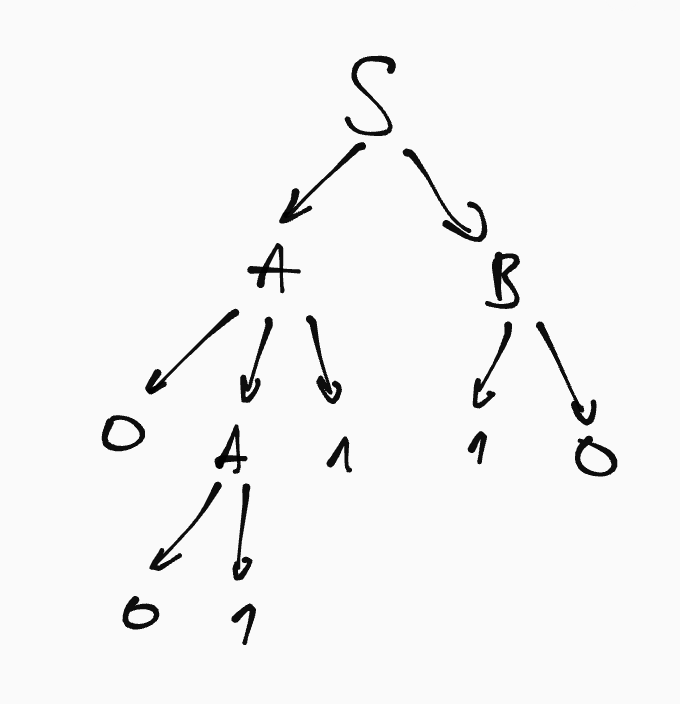
\includegraphics[width=0.5\linewidth]{04/4_1_a.png}


b)

$A$ generates $L_A = \{0^k1^k | k \geq{} 1\}$, $B$ generates $L_B = \{1^j0^j | j \geq{} 1\}$, and $S$ concatenates the two, so $L_S = \{0^k1^{k+j}0^j | j,k \geq{} 1\}$.\pagebreak
\subsection{Session 4, Exercise 2}

\lineparagraph{Exercise}

Consider

\begin{align*}
S \rightarrow& AS|A\\
A \rightarrow& 0A1|01
\end{align*}

\begin{enumerate}[(a)]
\item Give a parse tree and a leftmost derivation for word 01010011.
\item Determine the language generated by this grammar.
\end{enumerate}

\lineparagraph{Solution}\pagebreak
\subsection{Sessions 4 and 5, Exercise 3}

\lineparagraph{Exercise}

Give CF-grammars for the following languages. Are these unambiguous?

\begin{enumerate}[(a)]
\item $L = \{a^nb^{n+1}| n\geq{}0\}$
\item $L = \{a^nb^{2n} | n\geq{}0\}$
\item Palindromes over $\{a,b\}$
\item $L = \{a^ib^jc^k | (i = j \text{ or } i = k) \text{ and } i,j,k \geq{} 0\}$
\end{enumerate}

\lineparagraph{Solution}

(Multiple solutions can be correct here, we give one example for each.)

a)

\begin{align*}
    S \rightarrow& Tb\\
    T \rightarrow& aTb|\varepsilon
\end{align*}

$L_T = \{a^nb^n | n\geq{}1\}$, and $S$ just adds one more $b$ at the end. This language is unambiguous, since for \textbf{any} word in the grammar there is only a single possible (leftmost) derivation: we must always first use the $S \rightarrow Tb$ production rule, then the number of $a$'s and $b$'s determines the number of times the  $T \rightarrow aTb$ production rule is used, finally the $T \rightarrow \varepsilon$ must end the derivation.

Another good solution is $S \rightarrow aSb | b$, which does exactly the same thing with less rules.

b)

\begin{align*}
    S \rightarrow& aSbb|\varepsilon
\end{align*}

Since we now need twice as many $b$'s as $a$'s. This grammar is also unambiguous, since there is only one possible (leftmost) derivation for any word in the language: we use the $S \rightarrow aSbb$ as many times as there are $a$'s in the word, and then finally use $S \rightarrow \varepsilon$.

c)

\begin{align*}
    S \rightarrow& aSa | bSb | a | b |\varepsilon
\end{align*}

The matching characters in the palindromes are generated with rules $S \rightarrow aSa$ and $S \rightarrow bSb$, then if the palindrome is of odd length, the middle character is generated with rules $S \rightarrow a$ and $S \rightarrow b$, while if the palindrome is of even length, then no middle character is needed, so $S \rightarrow \varepsilon$ is used.

This grammar is unambiguous, since for any given palindrome, there is only one possible leftmost derivation for it: we read the input word from left-to-middle and when we see a character $a$ we must use production rule $S \rightarrow aSa$, when we see a $b$ we must use $S \rightarrow bSb$, then we take care of the middle character as we said before.

d)

\label{4f3d}

$L$ is the union of $L_1 = \{a^ib^ic^k | i,k \geq{} 0\}$ and $L_2 = \{a^ib^jc^i | i,j \geq{} 0\}$. So we can create a grammar by creating two independent grammars for $L_1$ and $L_2$ and combining them:

For $L_1$:
\begin{align*}
    X \rightarrow& TC\\
    T \rightarrow& aTb|\varepsilon\\
    C \rightarrow& cC|\varepsilon
\end{align*}

For $L_2$:
\begin{align*}
    Y \rightarrow& aYc|B\\
    B \rightarrow& bB|\varepsilon
\end{align*}

For $L=L_1\cup{}L_2$:

For $L_1$:
\begin{align*}
    S \rightarrow& X|Y\\
    X \rightarrow& TC\\
    T \rightarrow& aTb|\varepsilon\\
    C \rightarrow& cC|\varepsilon\\
    Y \rightarrow& aYc|B\\
    B \rightarrow& bB|\varepsilon
\end{align*}

This grammar is ambiguous, since the words of $a^ib^ic^i$ can be derived from both variable $X$ and variable $Y$ as well, so they have at least two leftmost derivations or parse trees.\pagebreak
\subsection{Session 4, Exercise 4}

\lineparagraph{Exercise}

Are the following grammars unambiguous? Are the languages generated by them unambiguous?

a)

\begin{align*}
S \rightarrow& aSa|bSb|aa|bb|a|b
\end{align*}

b)

\begin{align*}
S \rightarrow& TT|U \\
T \rightarrow& 0T|T0|\# \\
U \rightarrow& 0U00|\#
\end{align*}

\lineparagraph{Solution}\pagebreak
\subsection{Session 4, Exercise 5}

\lineparagraph{Exercise}

Let the alphabet be $\Sigma=\{0,1\}$, states of the pushdown automaton be $Q=\{A,B,C\}$, where $A$ is the start state, $C$ is the only accept state, let $Z$ be the start symbol of the stack. The transition function is the following:

\begin{align*}
    1.\text{ }\delta(A,0,\varepsilon) = \{(A,a)\}\\
    2.\text{ }\delta(A,1,\varepsilon) = \{(A, b)\}\\
    3.\text{ }\delta(A,\varepsilon,\varepsilon) = \{(B,\varepsilon)\}\\
    4.\text{ }\delta(B,0,a) = \{(B,\varepsilon)\}\\
    5.\text{ }\delta(B,1,b) = \{(B,\varepsilon)\}\\
    6.\text{ }\delta(B,\varepsilon, Z) = \{(C,\varepsilon)\}
\end{align*}

\begin{enumerate}[a)]
    \item Give the possible computations of the automaton on word 010.
    \item Does it accept word 0110?
    \item What is the language recognized by the automaton?
    \item Give a CF-grammar for this language.
\end{enumerate}

\lineparagraph{Solution}

a)

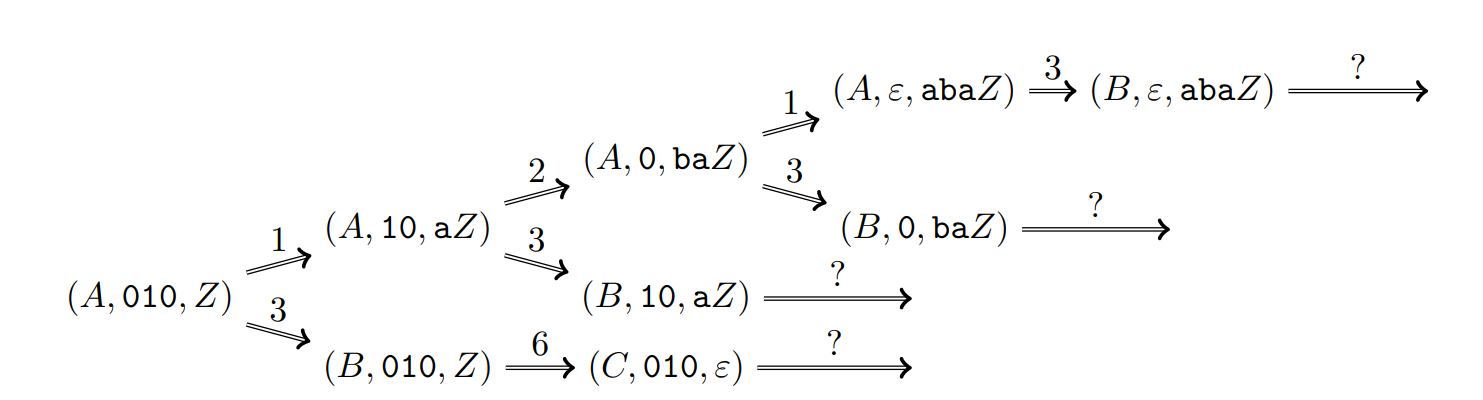
\includegraphics[width=\linewidth]{04/4_5_a.png}

b)

Yes, for example an accepting comutation (branch) is the following:


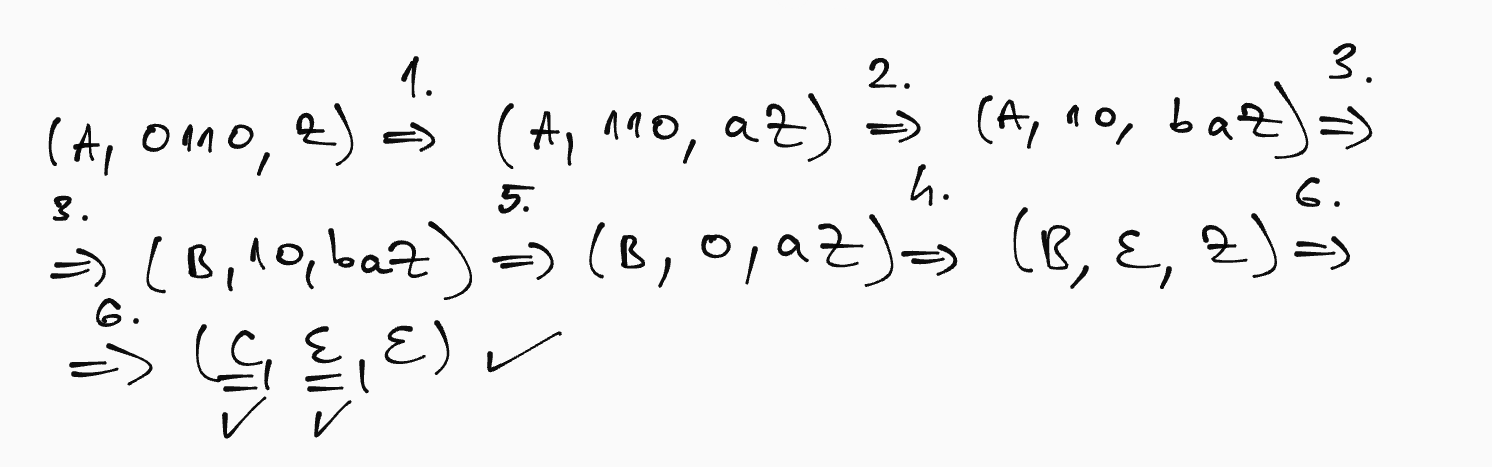
\includegraphics[width=\linewidth]{04/4_5_b.png}

c)

The language recognized is palindromes of odd length. These are accepted, since an accepting computation for these types of words will be: for the first half of the word transitions $1.$ and $2.$ will push the word ($0=a$, $1=b$) into the stack, then transition $3.$ will move to variable $B$, where the second (mirrored) half of the word will be compared to the first half on the stack using transitions $4.$ and $5.$. Since a stack is last-in-first-out, the comparisons will happen in the correct order. The stack can be emptied out this way and that allows for transition $6.$ to occur on the stack bottom symbol and move to the acceting $C$ state.

Words not in this language are rejected, since:
\begin{itemize}
    \item Only words of even length have a chance to be accepted, since the stack must be emptied out to move to the only accepting state and each character we put on the stack must have a pair that we use to remove it from the stack.
    \item Transition $3.$ must occur exactly at the middle of the word, for the same reason as stated above: if the word's length is $2n$, $n$ characters must be put on the stack, then move to state $B$, where $n$ characters must be removed from the stack. If the transition occurs too late, there will be remaining characters on the stack and we won't be able to move to state $C$, while if the transition occurs too early, the stack might be emptied out, however there will be remaining characters on he input so we could move to state $C$, however we won't accept since there are remaining characters on the input.
    \item If the word is not a palindrome, there must be at least one position where the character on it's mirrored position is wrong, either $a$ paired with a $b$ or $b$ paired with an $a$. This means, that when reading the stack back in state $B$, when we reach this position, we will have a wrong pairing: $0$ on the input with a character $b$ on the stack, or $1$ on the input with a character $a$ on the stack, for which no transition is defined from $B$, thus the machine will stop and the stack will not be empty, so we cannot move to state $C$ and $B$ is a rejecting state (plus, there will also be remaining input as well).
\end{itemize}

d)

\begin{align*}
    S \rightarrow& aSa | bSb | \varepsilon
\end{align*}

We have shown in previous exercises that this is indeed the grammar for palindromes of even length.\pagebreak
\subsection{Session 4, Exercise 6}

\lineparagraph{Exercise}

Construct a pushdown automaton for the language of palindromes.

\lineparagraph{Solution}

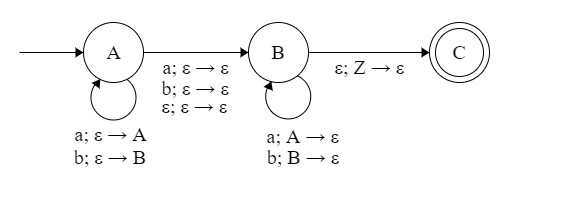
\includegraphics[width=0.5\linewidth]{04/4_6.png}

Proof:

States meaning:
\begin{itemize}
    \item State $A$ is used to read the first half of the word, and store it on the stack.
    \item State $B$ is used to read the second half of the word and compae it to the first half of the word on the stack.
    \item State $C$ can only be reached by emptying the stack out, so only palindromes can reach it.
\end{itemize}

Transitions:

\begin{itemize}
    \item State $A$'s loop transitions will store the corresponding characters on the stack.
    \item Transition from $A$ to $B$ takes care of the middle character, in case of an odd length palindrome, or is an epsilon transition in case of an even length palindrome.
    \item State $B$'s loop transitions will compare the second half of the word with the first half (mirrored, since a stack is a LIFO), and will only remove characters from the input and the stack if they match. If there is a character on the stack that doesn't match the PDA will halt in state $B$, which will reject.
    \item If the stack is emptied out we move to state $C$. In this case, if we read the entire input we can be sure that the word's first half matches the second half, and we will accept. If there are charaters remaining on the input, it means that not the entire word, only the prefix of the word was a palindrome, in which case the PDA correctly rejects, since there is still input remaining.
\end{itemize}

Accept / reject states:

The only accept state is state $C$ which can only be reached with no input remaining if the first half of the input is the mirror of the second half of the input. If a word is not a palindrome there won't be any accepting branch in the computation, all branches will end up in either $A$ (store the entire word), or $B$: start comparing too late, stack is not empty to move to $C$, or $C$ but with input remaining, since we started comparing too early.\pagebreak
\subsection{Session 4, Exercise 7}

\label{4_7}

\lineparagraph{Exercise}

Create pushdown automata for the following languages.
\begin{enumerate}[a)]
    \item $L_a = \{a^ib^jc^k | i,j,k \geq{} 0\text{ and }i+j = k\}$
    \item $L_a = \{a^ib^jc^k | i,j,k \geq{} 0\text{ and }j+k = i\}$
    \item $L_a = \{a^ib^jc^k | i,j,k \geq{} 0\text{ and }i+k = j\}$
\end{enumerate}


\lineparagraph{Solution}

a)

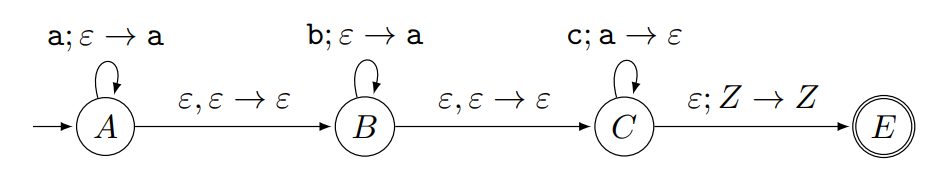
\includegraphics[width=\linewidth]{04/4_7_a.png}

TODO Proof

b)

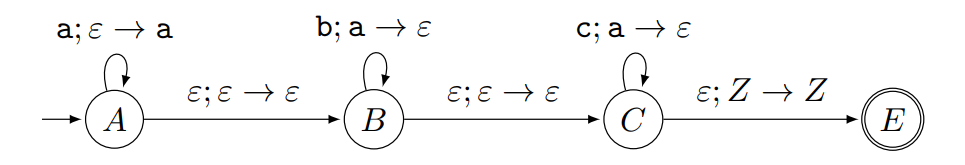
\includegraphics[width=\linewidth]{04/4_7_b.png}

TODO Proof

c)

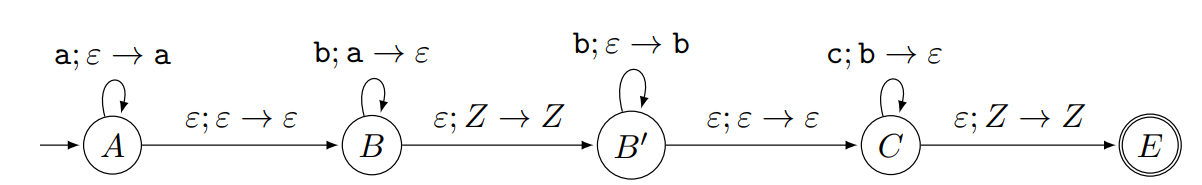
\includegraphics[width=\linewidth]{04/4_7_c.png}

TODO Proof

Note: c) is the tricky one, since we need the number of $a$'s plus the number of $c$'s to be equal to the number of $b$'s, but the $b$'s come in-between the $a$'s and the $c$'s. In this case we split the processing of $B$'s into two parts: in the first part we compare the number of $b$'s to the $a$'s that came before, while in the second part we store the number of $b$'s to be compared with the number of the upcoming $c$'s.

In this case we used non-determinism heavily, since the transition between $B$ and $B'$ must happen at the correct time for the calculation to work: one computational branch will time it correctly and that one can become an accepting branch (if everything else is correct with the word).\pagebreak
\subsection{Sessions 4 and 5, Exercise 8}

\lineparagraph{Exercise}

Create a pushdown automaton for the language of proper parenthesisations.

\lineparagraph{Solution}

Idea: correct parenthesisation can be checked by counting from left to right: start with $0$ and add $+1$ for every $($ encountered and $-1$ for every $)$ encountered. The parenthesisation is correct if the sum never drops below $0$ during the calculation (too many $)$ in that case at that point) and at the end it equals to $0$. A simple PDA can be constructed to do exactly this calculation.


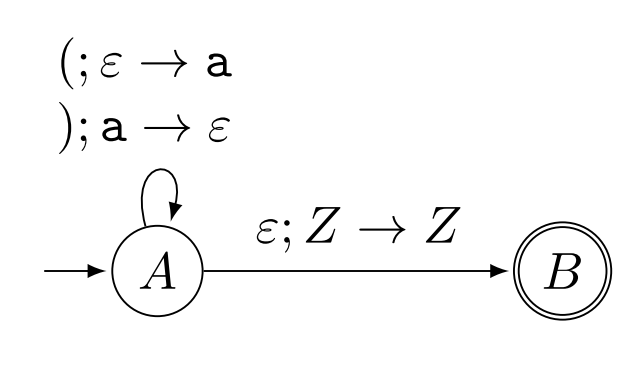
\includegraphics[width=0.4\linewidth]{04/4_8.png}

TODO Proof\pagebreak
\subsection{Sessions 4 and 5, Exercise 9}

\label{4_9}

\lineparagraph{Exercise}

Construct pushdown automata for the following languages.

\begin{enumerate}[a)]
\item $L_a = \{a^nb^m | 2n = m \geq{} 1\}$
\item $L_b = \{a^nb^m | 2n \geq{} m \geq{} n \geq{} 1\}$
\end{enumerate}

\lineparagraph{Solution}

a)

The first one is simpler, since we need to check for twice as many $b$'s as $a$'s. We can count the number of $a$'s in the stack with TWO tokens instead of one, so then the number of tokens in the stack must be equal to the number of $b$'s.

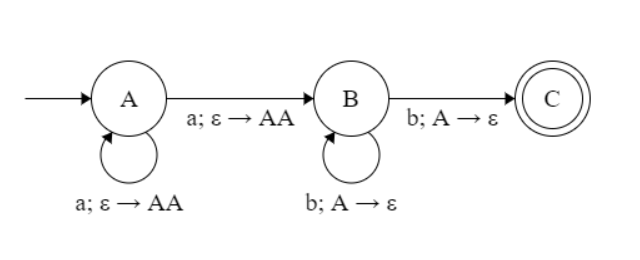
\includegraphics[width=0.5\linewidth]{04/4_9_a.png}

To enforce that the loops run at least once, due to the requirement that $n,m\geq{}1$ ($n\geq{}0.5$ is the same as $n\geq{}1$, since $n$ is an integer), we used non-epsilone transitions between the states, and copied the loop's transition to the existing transitions from the states as well.

TODO Proof

b)

The second one is more complex, since the number of $b$'s is now anywhere between $2n$ and $n$! How do we enforce $2n \geq{} m \geq{} n$? We just did it with $2n = m$, also if it were only $n = m$, we could replace the $a; \varepsilon \rightarrow AA$ transitions with  $a; \varepsilon \rightarrow A$ transitions. But how do we check for in-between these two numbers?

We will rely on non-determinism again:

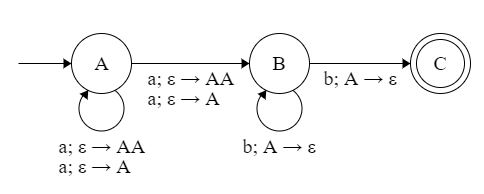
\includegraphics[width=0.5\linewidth]{04/4_9_b.png}

We use both $a; \varepsilon \rightarrow A$ and $a; \varepsilon \rightarrow AA$. The PDA will nondeterministically use either the first or the second transition and push either 1 or 2 $A$'s on the stack. So the number of $A$'s on the stack will be anywhere between $2n$ and $n$, and there will exist a computational branch (if the word is in the language) where their number will be equal to $m$ and the word will be accepted.\pagebreak
\subsection{Sessions 4 and 5, Exercise 10}

\lineparagraph{Exercise}

TODO

\lineparagraph{Solution}

TODO\pagebreak
\subsection{Sessions 4 and 5, Exercise 11}

\lineparagraph{Exercise}

TODO

\lineparagraph{Solution}

TODO\pagebreak
\subsection{Session 4, Exercise 12}

\lineparagraph{Exercise}

TODO

\lineparagraph{Solution}

TODO\pagebreak

\section{Turing-machines}
\subsection {Session 6, Exercise 1}

Same as \ref{6f3}.\pagebreak
\subsection{Session 6, Exercise 2}

\lineparagraph{Exercise}

A 2-szalagos $M$ Turing-gép átmeneti függvényét a következő táblázat írja le, ahol * jelöli a szalagon az üres jelet és $q_{0}$ a kezdő állapotot:

\begin{tabular}{|c|c|c||cc|cc|c|}
\hline állapot & 1. szalag & 2. szalag & 1. szalag & 2. szalag & új állapot \\
\hline$q_{0}$ & 0 & $*$ & 0 & $\mathrm{H}$ & $\mathrm{X}$ & $\mathrm{J}$ & $q_{1}$ \\
& 1 & $*$ & 1 & $\mathrm{H}$ & $\mathrm{X}$ & $\mathrm{J}$ & $q_{1}$ \\
& $*$ & $*$ & $*$ & $\mathrm{H}$ & $*$ & $\mathrm{H}$ & $q_{5}$ \\
\hline$q_{1}$ & 0 & $*$ & 0 & $\mathrm{~J}$ & 0 & $\mathrm{~J}$ & $q_{1}$ \\
& 1 & $*$ & 1 & $\mathrm{~J}$ & 1 & $\mathrm{~J}$ & $q_{1}$ \\
& $*$ & $*$ & $*$ & $\mathrm{H}$ & $*$ & $\mathrm{~B}$ & $q_{2}$ \\
\hline$q_{2}$ & $*$ & 0 & $*$ & $\mathrm{H}$ & 0 & $\mathrm{~B}$ & $q_{2}$ \\
& $*$ & 1 & $*$ & $\mathrm{H}$ & 1 & $\mathrm{~B}$ & $q_{2}$ \\
& $*$ & $\mathrm{X}$ & $*$ & $\mathrm{~B}$ & $\mathrm{X}$ & $\mathrm{J}$ & $q_{3}$ \\
\hline$q_{3}$ & 0 & 0 & 0 & $\mathrm{H}$ & 0 & $\mathrm{~J}$ & $q_{4}$ \\
& 1 & 1 & 1 & $\mathrm{H}$ & 1 & $\mathrm{~J}$ & $q_{4}$ \\
\hline$q_{4}$ & 0 & 0 & 0 & $\mathrm{~B}$ & 0 & $\mathrm{H}$ & $q_{3}$ \\
& 0 & 1 & 0 & $\mathrm{~B}$ & 1 & $\mathrm{H}$ & $q_{3}$ \\
& 1 & 0 & 1 & $\mathrm{~B}$ & 0 & $\mathrm{H}$ & $q_{3}$ \\
& 1 & 1 & 1 & $\mathrm{~B}$ & 1 & $\mathrm{H}$ & $q_{3}$ \\
& 0 & $*$ & 0 & $\mathrm{H}$ & $*$ & $\mathrm{H}$ & $q_{5}$ \\
& 1 & $*$ & 1 & $\mathrm{H}$ & $*$ & $\mathrm{H}$ & $q_{5}$ \\
\hline
\end{tabular}

(a) Mi a 2. szalag tartalma, amikor a gép $q_{2}$ állapotba kerül?

(b) Mi az $L(M)$ nyelv, ha $q_{5}$ az egyetlen elfogadó állapot?

(c) Legfeljebb hány lépést tehet a gép egy $n$ hosszú bemeneten, mielőtt megáll?

\lineparagraph{Solution}

Nézzük, mi történik:

$q_{0}:$ Ha nem üres a bemenet, akkor egy $X$ kerül a 2. szalagra (ez jelzi majd a szalag elejét).

$q_{1}$ : Lemásolja az 1. szalagon talált karaktert a 2. szalagra. Akkor lép csak ki innen, ha a bemenet végére ért (ekkor, ha az elsö szalagon a $w$ szó van, akkor a 2. szalagon $X w$ ). Ilyenkor következik a $q_{2}$ állapot, ahova úgy lépünk át, hogy az 1. szalagon maradunk az első üres mezón, a 2. szalagon visszalépünk az utolsónak írt karakterre.

$q_{2}:$ Az első szalagon nem mozdulunk, mialatt visszamegyünk a 2 . szalag elejére. Végül úgy lépünk át $q_{3}$-ba, hogy az 1. szalagon egyet visszalépünk (az utolsó nem üres mezóre), a 2. szalagon egyet elóre lépünk (az elsö nem $X$ karakterre). $q_{3}$ : Ha ugyanazt látjuk mindkét szalagon, akkor az elsőn nem mozdulunk, a másodikon egyet előre lépünk és átkerülünk $q_{4}$-be. (Elsớ alkalommal tehát az 1. szalag utolsó és a 2. szalag $X$ utáni elsö karakterét, azaz a $w$ első és utolsó karakterét hasonlítjuk össze. Ha nem egyeznek, akkor ebben a nem elfogadó állapotban leállunk.)

$q_{4}$ : Ha nem értük el a 2. szalag végét, akkor semmit nem változtatva az 1. szalagon visszafelé lépünk egyet, a 2. szalagon helyben maradunk és a $q_{3}$-ban folytatjuk. Azaz a $q_{3}$-beli hasonlítás és a $q_{4}$-beli lépés felváltva addig történik, amíg el nem érünk a 2. szalag végére. Ekkor átlépünk a q elfogadó állapotba és a számítás sikeresen véget ért.

Az üres szón érdemi munka nélkül egyból átjutunk az elfogadó állapotba.

(a) Ha $w$ a bemeneti szó, akkor $X w$.

(b) A palindromok nyelve.

(c) Egy $n$ hosszú palindromon a lépések száma: $1+(n+1)+(n+1)+(2 n-1)+1=4 n+3$. Ha a szó nem palindrom, akkor elóbb elakadhat (de a másolás és a 2. szalag elejére visszalépegetés akkor is megtörténik, $2 n+3$ lépés akkor is lesz, amennyiben $n>0)$.\pagebreak
\subsection {Session 6, Exercise 3}

\label{6_3}

\lineparagraph {Exercise}

The following table contains the transition function of a 2-tape Turing machine, where $*$ is the blank symbol on the tapes, and $q_0$ is the start state.

\begin{center}
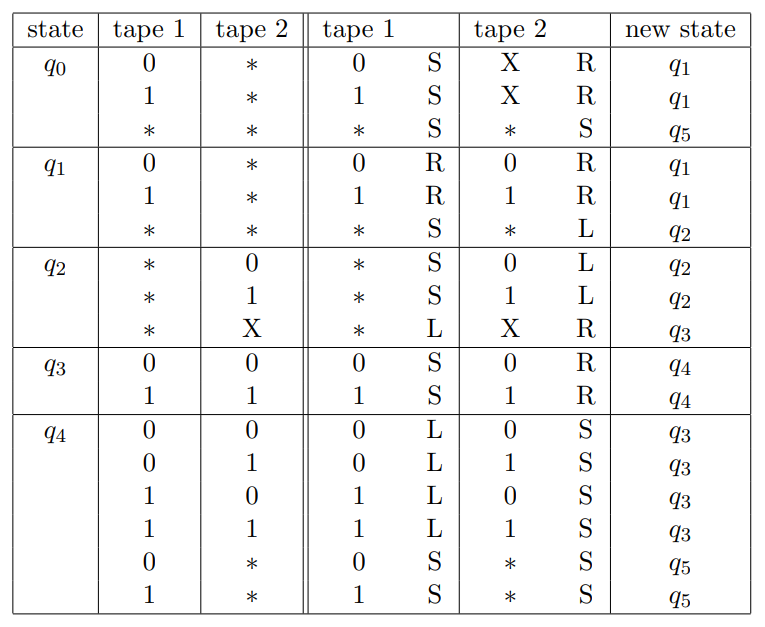
\includegraphics[width=0.7\linewidth]{06/6_3_task.png}
\end{center}

\begin{enumerate}[a)]
    \item What is the content of tape 2 when the machine moves to state $q_2$?
    \item What is the language $L(M)$ if the only accept state is $q_5$?
    \item At most how many steps are done by the machine on an input of length $n$ before it stops?
\end{enumerate}

\lineparagraph {Solution}

To see a little bit easier what this TM does, I converted it line-by-line to the below form:

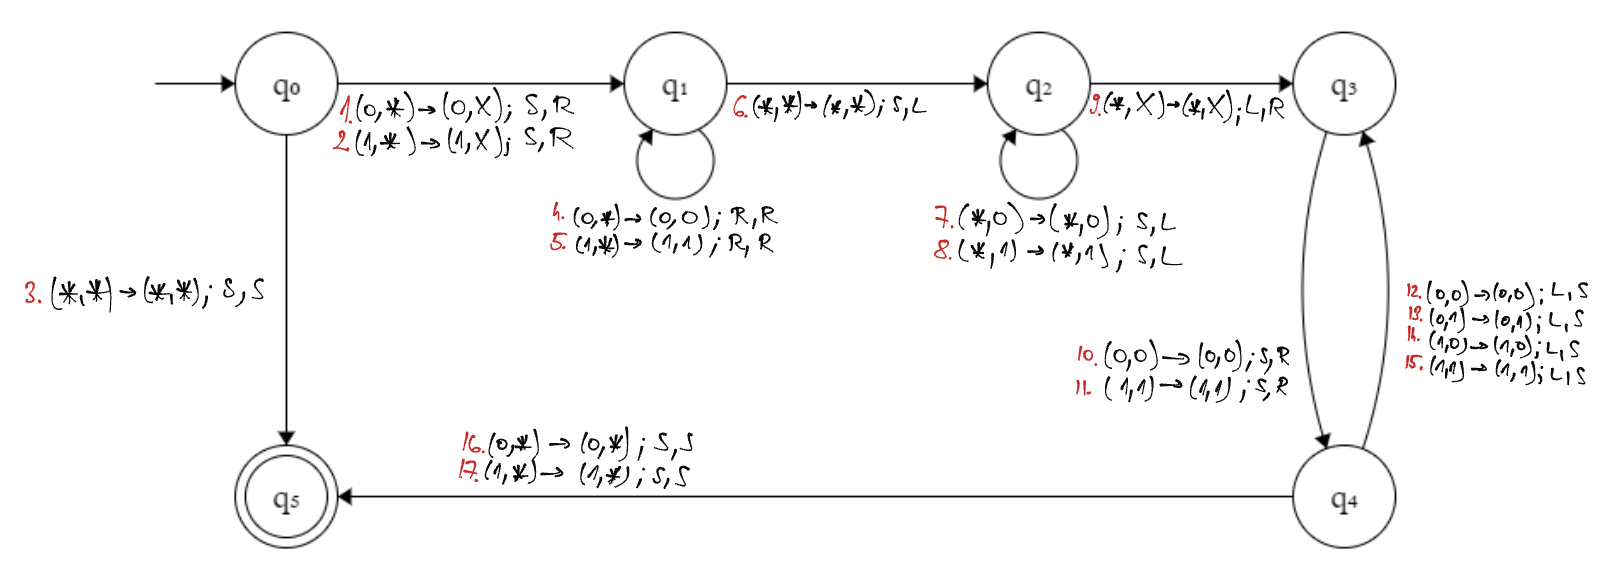
\includegraphics[width=\linewidth]{06/6_3_canvas.png}

What this does:
\begin{itemize}
    \item Transition 3: This one handles the empty string input and immediately moves to the accept state $q_5$. So the empty string is accepted. So the empty string is accepted in $1$ step. For any other input, the following happens:
    \item Transitions 1-2: They put down an $X$ character at the beginning of the second tape. This $X$ will be used later to make sure that the head does not fall of the tape (moving from the first position to the left would cause the head to fall off, this $X$ is there so we can detect it and make sure no transition is defined that moves the 2nd head to the left when it reads an $X$). This is $1$ step.
    \item Transitions 4-5: They copy the first tape's contents to the second tape. This is $n$ steps if the input is of length $n$.
    \item Transition 6: When the on the first tape the head is at the end of the input word (sees the $* =$ empty cell character we move to state $q_2$ and we position the second head on the last character of the copied input. (While the first head remains on the $* =$ empty cell after the input.) This is $1$ step.
\end{itemize}

a) When we move to state $q_2$ the contents of tape $2$ will be the character $X$ at the beginning, then the input word copied afterwards.

\begin{itemize}
    \item Transitions 7-8: The first head stays on the same $*$ cell, while the second had moves to the left until it finds the character $X$ (beginning of the second tape). This is $n$ steps if the input is of length $n$.
    \item Transition 9: The first head is positioned at the end of the input word, while the second head is positioned at the beginning of the (copied) input word. This is $1$ step.
    \item Transitions 10-15: Together these make $2n$ steps for an input word of length $n$, see explanation below:
    \begin{itemize}
        \item Transitions 10-11: These compare the two strings (the input word twice, on the first tape from right to left and on the second tape from left to right). However, the first head is not moved immediately to the left. This is because the first head could fall off the first tape, since there is no protective $X$ there. We cannot recklessly move to the left.
        \item Transitions 12-15: Instead we lag behind the second head and make sure that the second head reads either a $0$ or a $1$ (and the first head can read $0$ or $1$ as well), which means that the word has not yet ended! (The second head would read $*$ here when the word ends.) This means that it is \textbf{safe} to move the first head to the left, since it is not yet at the beginning of the tape, so we move.
    \end{itemize}
    \item Transitions 16-17: Finally, when the second head reads the empty cell, it means that the word has ended (and has been successfully compared), so we can move to $q_5$. We make sure that we \textbf{DO NOT} move the first head to the left in this step, since it would fall off. Since the first head could be on a character $0$ or a $1$ we need to define 2 transitions to cover all possibilities. We move to $q_5$ here. This is $1$ step.
\end{itemize}

Together the number of steps for a successfull computation has been (for a non-empty input):

\begin{itemize}
    \item Transitions 1-2: $1$ step.
    \item Transitions 4-5: $n$ steps.
    \item Transition 6: $1$ step.
    \item Transitions 7-8: $n$ steps.
    \item Transition 9: $1$ step.
    \item Transitions 10-15: $2n$ steps.
    \item Transitions 16-17: $1$ step.
\end{itemize}

At most $4n+4$, but keep in mind that for a rejecting computation the number of steps is smaller, depending on where it halts in transitions 10-15. (At least $2n+3$ steps, since copying and moving the second head back to the first position will be done regardless of rejecting / accepting.)\pagebreak
\subsection{Session 6, Exercise 4}

\lineparagraph{Exercise}

Adjon Turing-gépet a $\left\{w \# w: w \in\{0,1\}^{*}\right\}$ nyelvhez! Adjon felsó becslést a Turing-gép lépésszámának nagyságrendjére!

\lineparagraph{Solution}

Lássunk előbb egy 2 szalagos gépet! Az ötlet, hogy a 2. szalagra lemásoljuk a szó elejét (az $m=$ másolás állapotban). A # jelhez érve átlépünk egy újabb $v$ állapotba, amivel visszamegyünk a 2 . szalag elejére (v=vissza állapot), és onnan kezdve majd ezt hasonlítjuk az 1. szalagon levő szó második feléhez ( $h$ állapot). Arra most is figyelni kell, hogy a 2. szalag elejére tegyünk egy jelet $(s \rightarrow m)$, hogy visszafelé jövet tudjuk, hol az eleje.

Azt az esetet is kezelni kell, ha a $w$ az üres szó, az egyetlen # karakterból álló bemenetet is el kell fogadni, ez történik az $u 1$ és $u 2$ állapot segítségével.

$(0, *) \rightarrow(0, X), \mathrm{H}, \mathrm{J}$

$(0, *) \rightarrow(0, X), \mathrm{H}, \mathrm{J}$
$(1, *) \rightarrow(1, X), \mathrm{H}, \mathrm{J}$

![](https://cdn.mathpix.com/cropped/2022_03_23_c86c88fa24d5c87623acg-2.jpg?height=108&width=1046&top_left_y=1271&top_left_x=109)

$(0, *) \rightarrow(0,0), \mathrm{J}, \mathrm{J} \quad(\#, 0) \rightarrow(\#, 0), \mathrm{H}, \mathrm{B} \quad(0,0) \rightarrow(0,0), \mathrm{J}, \mathrm{J}$

$\begin{array}{ll}(1, *) \rightarrow(1,1), \mathrm{J}, \mathrm{J} & (\#, 1) \rightarrow(\#, 1), \mathrm{H}, \mathrm{B} \quad(1,1) \rightarrow(1,1), \mathrm{J}, \mathrm{J}\end{array}$

![](https://cdn.mathpix.com/cropped/2022_03_23_c86c88fa24d5c87623acg-2.jpg?height=128&width=291&top_left_y=1476&top_left_x=142)

Lépésszám: Az $n$ hosszú bemeneteken az $m, v$ és $h$ állapotok bármelyikében legfeljebb $n$ lépést töltünk, ezeken kívül csak konstans sok lépés van, tehát a lépésszám $O(n)$. (Könnyú látni, hogy az elfogadott szavakra $\Theta(n)$ is igaz. Miért nem igaz ez minden bemenetre?)

Egy másik megoldás 1 szalaggal: most azt csináljuk, hogy oda-vissza mozogva a szalagon hasonlítjuk a párokat, amiken túl vagyunk, azokat átírjuk $X$-re. Részletesebben: az első karaktert felülírjuk, és attól függóen, hogy ez 0 vagy 1 volt, megyünk az $n$ vagy e állapotba. A két ágon hasonlóan járunk el, az $n$ és $e$ állapotban elmegyünk a # jelig, majd a bemenet második felében átlépjük az esetleges $X$ jeleket (ln, le). Ha az ez után jövö elsố karakter megfelel annak, amit várunk (az $n$ ágon o, az e ágon 1), akkor a szó eddig jó, ezt a karaktert felülírjuk, és visszamegyünk az $X$-eken a # jelig, ami után a # állapotban átlépkedünk a szó elsố felében még megmaradt 0 és 1 karaktereken. Amikor elérjük az elsố $X$ jelet, akkor az s állapotból folytathatjuk a következố karakterpár ellenórzését. Ha ide érve a # karaktert látjuk, akkor a szó elsố felét feldolgoztuk. Ha ilyenkor a második felében sem maradt $X$-en kívül semmi, akkor elfogadunk. (Ugyanez történik, ha $w=\varepsilon$ ).

![](https://cdn.mathpix.com/cropped/2022_03_23_c86c88fa24d5c87623acg-3.jpg?height=584&width=950&top_left_y=415&top_left_x=91)

A lépésszám becsléséhez elég azt észrevenni, hogy egyrészt minden állapotban egyfolytában legfeljebb $n$ lépésig maradunk (hiszen a nem $X$ karakterek száma minden körben eggyel csökken), másrészt az $s$ állapotba legfeljebb $n$-szer térünk vissza. Ezért a lépésszám összesen $O\left(n^{2}\right)$.\pagebreak
\subsection {Session 6, Exercise 5}

\lineparagraph {Exercise}

Let $\Sigma = \{0, 1, +\}$. Sketch a Turing machine that on an input of form $x + y$ where $x$, $y \in \{0, 1\}^*$ are nonempty bitstrings stops in finite time and when it stops on its 5th tape the sum of binary numbers x and y stands. Give an upper bound on its running time.

\lineparagraph {Solution}

\begin{itemize}
    \item Mark the beginning of tapes 2,3,4 tapes with an $X$.
    \item We first copy the input up until the $+$ character to the second tape. If no $+$ is found the input is rejected.
    \item We then copy the second part of the input after the $+$ character until the first emtpy cell. If there is another $+$ found, we reject.
    \item Now step with heads $2$ and $3$ 1 step backwards, to stand on the least significant bit of both $x$ and $y$.
    \item We do the method of summing two numbers we learnt in primary school. We store the current carry bit in our current state: $C_0$ and $C_1$. There are $8$ ($12$) possibilities:
    \begin{itemize}
        \item If the current state is $C_0$:
        \begin{itemize}
            \item If both heads see a $0$: We write a $0$ on the 4th tape and stay in $C_0$.
            \item If one head sees a $0$ or an empty cell and the other a $1$: We write a $1$ on the 4th tape and stay in state $C_0$.
            \item If both heads see a $1$: We write a $0$ on the 4th tape and move to state $C_1$.
            \item If both heads see an empty cell: Computation is done here, move to the copying stage.
        \end{itemize}
        \item If the current state is $C_1$:
        \begin{itemize}
            \item If both heads see a $0$: We write a $1$ on the 4th tape and move to $C_0$.
            \item If one head sees a $0$ or an empty cell and the other a $1$: We write a $0$ on the 4th tape and stay in state $C_1$.
            \item If both heads see a $1$: We write a $1$ on the 4th tape and stay in state $C_1$.
            \item If both heads see an empty cell: Since we still have a carry bit, we write that down on the 4th tape, then computation is done here, move to the copying stage.
        \end{itemize}
    \end{itemize}
    \item And if the current head saw a $0$ or a $1$ we move it to the left for both tape $2$ and $3$, while the head on tape $4$ moves to the right.
    \item After finishing with the computation we will have the required sum on the 4th tape, however the least significant bit will be on the first place. We need to reverse it.
    \item We can done this by copying from the current (last) position on the 4th tape to the 5th, by moving the 4th head to the left and the 5th head to the right, step-by-step.
\end{itemize}

This computation is done in $O(n)$, since copying to tape 2 and 3 is done in $O(n)$, then summing is done in $O(n)$ and finally reversal is also done in $O(n)$. (The resulting sum's length will not exceed the sum of the input $x$ and $y$ number's length in binary form.)\pagebreak
\subsection {Session 6, Exercise 6}

\lineparagraph {Exercise}

Let $L_r$ be an arbitrary regular language and let $L_c$ be an arbitrary CF language.
\begin{enumerate}
    \item Show an example when $L_r \cap L_c$ is not regular.
    \item Prove that $L_r \cap L_c$ is always context-free.
    \item Show an example when $L_1$ and $L_2$ are both context-free but $L_1 \cap L_2$ is not.
\end{enumerate}

\lineparagraph {Solution}

a)

For example if we take $L_r = \Sigma^*$, which is regular. Then, we take a known non-regular, but CF language, $L_c = \{a^nb^n | n \geq{} 0\}$. Ther instersection is $L_c$ itself, which is not regular, but CF.

b) If $L_r$ is regular, there exists a DFA that accepts it, let's call this $M_r$. Then, since $L_c$ is CF, there exists a PDA that accepts it, let's call this $M_c$. To show that $L_r \cap L_c$ is CF we construct a PDA from $M_r$ and $M_c$ that accepts it.

The main idea is to take all the possible pairs of states, where one state comes from $M_r$ and the other from $M_c$. For a given input character, we define the transition function, so that ''it keeps track of what's happening in both $M_r$ and $M_c$ at the same time'', for each statepair $(q_r, q_c)$, by checking what $M_r$ would do for the given input character in state $q_r$ and what would $q_c$ do, and moving to that statepair (or, since the PDA can have a set of possible states it moves into, the set of all statepairs).

We keep track of what's happening in $M_c$'s stack in the stack we have (this is why we cannot do this for two CF-languages, we would need to keep track of two stacks).

The starting statepair is going to be the statepair which contains the starting states from their respective machines.

The accepting statepairs will be the ones for which both states accept in their respective machines, since we need $L_r \cap L_c$.

The PDA constructed in this way will accept $L_r \cap L_c$, which means that the language is CF.

c)

These languages are both CF:

$L_1 = \{a^nb^nc^k | n,k \geq{} 0\}$ (Number of $a$'s and $b$'s is equal.)

$L_2 = \{a^ib^jc^j | i,j \geq{} 0\}$ (Number of $b$'s and $c$'s is equal.)

(See \ref{4_3_d} for a CF-grammar for $L_1$, and based on that $L_2$ can be constructed in a similar manner.)

$L_1 \cap L_2 = \{a^nb^nc^n\}$  (Number of $a$'s and $b$'s and $c$'s is equal.)

Which is known to be non-CF. (The idea behind this is that we would need to use the stack to keep track of the number of $a$'s, but we would throw them out when comparing them with the number of $b$'s and there will be nothing left to compare to when the $c$'s come. The formal proof is more complicated and outside of the scope of this class.)\pagebreak
\subsection{Session 6, Exercise 7}

\lineparagraph{Exercise}

Legyen $L_{r}$ egy tetszóleges reguláris nyelv és legyen $L_{c}$ egy tetszöleges környezetfüggetlen nyelv.

(a) Mutasson olyan példát, amikor $L_{r} \cap L_{c}$ nem reguláris!

(b) Igazolja, hogy $L_{r} \cap L_{c}$ mindig környezetfüggetlen!

(c) Mutasson olyan példát, amikor $L_{1}$ és $L_{2}$ is környezetfüggetlen, de $L_{1} \cap L_{2}$ nem az!

\lineparagraph{Solution}

(a) Ha $L_{r}=\{\mathrm{a}, \mathrm{b}\}^{*}$ és $L_{c}=\left\{a^{n} b^{n}: n \geq 0\right\}$, akkor $L_{r} \cap L_{c}=L_{c}$, ami nem reguláris.

(b) Legyen $M_{1}=\left(Q_{1}, \Sigma, q_{1}, F_{1}, \delta_{1}\right)$ egy DVA az $L_{r}$ nyelvhez, és $M_{2}=\left(Q_{2} . \Sigma, \Gamma, q_{2}, Z_{0}, F_{2}, \delta_{2}\right)$ egy veremautomata az $L_{c}$ nyelvhez. A kettőból elkészíthetjük azt az $M$ veremautomatát, amelynek állapothalmaza $Q_{1} \times Q_{2}$, kezdőállapota $\left(q_{1}, q_{2}\right)$, elfogadó állapotainak halmaza $F_{1} \times F_{2}$, az átmeneteiben az állapot elsó koordinátájában $\delta_{1}$ szerint lép, a másodikban $\delta_{2}$ szerint. Amennyiben a veremautomata nem olvas a bemenetrôl, akkor az állapot első koordinátája nem változik ( $M_{1}$ nem lép). Ha a veremautomata nem tud lépni, akkor $M$ számítása elakad. A veremben mindig történjen az, ami az $M_{2}$ megfeleló lépésében történik.

Ez az automata lényegében párhuzamosan futtatja az $M_{1}$ és $M_{2}$ automatát, akkor fogad el, ha mindkettő elfogadó.

(c) $\mathrm{Az} L_{1}=\left\{\mathrm{a}^{n} \mathrm{~b}^{n} \mathrm{c}^{k}: n \geq 0\right\}$ és $L_{2}=\left\{\mathrm{a}^{n} \mathrm{~b}^{k} \mathrm{c}^{n}: n \geq 0\right\}$ nyelvek környezetfüggetlenek (lásd 5 . gyak. 1(b)), a metszetük az $\left\{\mathrm{a}^{n} \mathrm{~b}^{n} \mathrm{c}^{n}: n \geq 0\right\}$ nyelv, ami nem $\mathrm{CF}$.

(A (b)-ben vázolt konstrukció az automatákra most azért nem múködik, mert két vermet kellene eggyel szimulálni.)\pagebreak
\subsection{Session 6, Exercise 8}

\lineparagraph{Exercise}

Legyen $\Sigma=\{1\}$, az 1-szalagos Turing-gép átmeneti függvénye $\delta\left(q_{0}, 1\right)=\left(q_{1}, 1, J\right), \delta\left(q_{0}, *\right)=\left(q_{2}, *, J\right)$, $\delta\left(q_{1}, 1\right)=\left(q_{3}, 1, J\right), \delta\left(q_{3}, 1\right)=\left(q_{0}, 1, J\right)$, kezdő állapot a $q_{0}$, elfogadó a $q_{3}$. Mi a gép által elfogadott nyelv?

\lineparagraph{Solution}

Vegyük észre, hogy ez a Turing-gép nem változtatja meg a szalag tartalmát, mindig az ott talált karaktert írja vissza és mindig tovább lép jobbra.

Az üres szóra a $\delta\left(q_{0}, *\right)=\left(q_{2}, *, J\right)$ szabállyal $q_{2}$-be lép, és mivel ott nincs átmenet definiálva, megáll. A q ${ }_{2}$ nem elfogadó állapot, ezért nem fogadja el az üres szót.

Az 1 karakterek hatására a $q_{0}, q_{1}, q_{3}$ állapotokon mozog körbe-körbe. Akkor fogad el, ha ez a $q_{3}$-ban áll le, azaz az elfogadott nyelv: $\left\{1^{k}: k \equiv 2(\bmod 3)\right\}$.

(És mi a nyelv, ha $\{0,1\}$ az ábécé?)\pagebreak
\subsection{Session 6, Exercise 9}

\lineparagraph{Exercise}

Legyen $\Sigma=\{0,1,+,=\}$. Vázoljon egy Turing-gépet ahhoz a nyelvhez, amelyik az olyan $x+y=z$ alakú szavakból áll, ahol $x, y, z \in\{0,1\}^{*}$ nem üres bitsorozatok, és ha ezeket binárisan felírt számoknak tekintjük, akkor valóban $z$ az $x$ és $y$ összege. Adjon becslést a Turing-gép lépésszámára!

\lineparagraph{Solution}

Az egyszerúség kedvéért használjunk 4 szalagot. Elöször a bemenetrơl a + -ig terjedô részt $(x)$ a szokott módon lemásoljuk a 2. szalagra (elơtte megjelölve a szalag elejét). Majd az = -ig a következö részt (y) hasonlóan átmásoljuk a 3. szalagra. Álljunk vissza a fejjel a 2. és 3. szalag utolsó nem üres mezójére (azaz $x$ és $y$ utolsó bitjére), hiszen az összeadát az utolső bitnél jó kezdeni.

A 4. szalagra írjuk az összeget a szám végéról kezdve. Az összeadásnál két állapotot használunk, az egyik jelképezi, hogy volt átvitel az elơzó számjegy összeadásából, a másik meg, hogy nem volt. Ennek megfelelöen a két állapotban mást-mást írunk a 4. szalagra ugyanannál az olvasott karakterpárnál.

Ha az összeadás véget ért, össze lehet hasonlítani az eredményt, azaz a 4. szalag tartalmát visszafelé, az első szalagon az $=$ utáni $(z)$ résszel.

(Az összeg felírását el is kerülhetjük, ha a keletkezö karaktereket egyből a z rész megfelelő karakterével összehasonlítjuk.)\pagebreak

\end{document}
